%%
%% ACS project dissertation template.
%%
%% Currently designed for printing two-sided, but if you prefer to
%% print single-sided just remove ",twoside,openright" from the
%% \documentclass[] line below.
%%
%%
%%   SMH, May 2010.


\documentclass[a4paper,12pt,twoside,openright]{report}


%%
%% EDIT THE BELOW TO CUSTOMIZE
%%

\def\authorname{Tom M. Read Cutting\xspace}
\def\authorcollege{Downing College\xspace}
\def\authoremail{tr395@cam.ac.uk}
\def\dissertationtitle{Heterogeneous type checking in multi-language CPU-GPU systems}
\def\wordcount{6461}
\def\totalloccount{13000 }
\def\compilerloccount{12000 }


\usepackage{array,color,epsfig,float,inconsolata,graphicx,hyperref,listings,parskip,setspace,tabularx,tabu,textcomp,xspace}
\graphicspath{ {images/} }

\newfloat{lstfloat}{htbp}{lop}
\floatname{lstfloat}{Listing}
\def\lstfloatautorefname{Listing} % needed for hyperref/auroref

\definecolor{codegreen}{rgb}{0,0.6,0}
\definecolor{codegray}{rgb}{0.5,0.5,0.5}
\definecolor{codepurple}{rgb}{0.58,0,0.82}
\definecolor{backcolour}{rgb}{0.95,0.95,0.92}
\lstdefinestyle{mystyle}{
    backgroundcolor=\color{backcolour},
    commentstyle=\color{codegreen},
    keywordstyle=\color{magenta},
    numberstyle=\tiny\color{codegray},
    stringstyle=\color{codepurple},
    basicstyle=\ttfamily\footnotesize,
    breakatwhitespace=false,
    breaklines=true,
    captionpos=b,
    keepspaces=true,
    numbers=left,
    numbersep=5pt,
    showspaces=false,
    showstringspaces=false,
    showtabs=false,
    tabsize=2
}

\lstset{style=mystyle}

%% START OF DOCUMENT
\begin{document}


%% FRONTMATTER (TITLE PAGE, DECLARATION, ABSTRACT, ETC)
\pagestyle{empty}
\singlespacing
% title page information
\begin{titlepage}

\begin{center}
\noindent
\huge
\dissertationtitle \\
\vspace*{\stretch{1}}
\end{center}

\begin{center}
\noindent
\huge
\authorname \\
\Large
\authorcollege      \\[24pt]

\includegraphics{CUni3.eps}
\end{center}

\vspace{24pt}

\begin{center}
\noindent
\large
{\it A dissertation submitted to the University of Cambridge \\
in partial fulfilment of the requirements for \\
Computer Science Tripos, Part III}
\vspace*{\stretch{1}}
\end{center}

\begin{center}
\noindent
University of Cambridge \\
Department of Computer Science and Technology \\
William Gates Building  \\
15 JJ Thomson Avenue    \\
Cambridge CB3 0FD       \\
{\sc United Kingdom}    \\
\end{center}

\begin{center}
\noindent
Email: \authoremail \\
\end{center}

\begin{center}
\noindent
\today
\end{center}

\end{titlepage}

\newpage
\vspace*{\fill}

\onehalfspacing
\newpage
{\Huge \bf Declaration}

\vspace{24pt}

I \authorname of \authorcollege, being a candidate for the M.Phil in
Advanced Computer Science, hereby declare that this report and the
work described in it are my own work, unaided except as may be
specified below, and that the report does not contain material that
has already been used to any substantial extent for a comparable
purpose.

\vspace{24pt}
Total word count: \wordcount

\vspace{60pt}
\textbf{Signed}:

\vspace{12pt}
\textbf{Date}:


\vfill

This dissertation is copyright \copyright 2018 \authorname.
\\
All trademarks used in this dissertation are hereby acknowledged.



\newpage
\vspace*{\fill}

\singlespacing
\newpage
{\Huge \bf Acknowledgements}
\vspace{24pt}

I would like to thank everyone who supported me through a difficult year, and
ensured that I saw this project through to the end.

I would like to thank Nicholas Timmons for providing early feedback on project
ideas, and helping me navigate the messy world of graphics programming.

I would like to especially thank my supervisor Professor Alan Mycroft, who has
been both understanding and accommodating, in addition to providing the honest
and wise feedback necessary for me to focus my thoughts.

\newpage
\vspace*{\fill}

\singlespacing
\newpage
{\Huge \bf Abstract}
\vspace{24pt}

% 1 sentence setting out the the scene, future holds promise.

% this thesis sets scene then give contributions.

% TODO: so step back and look at heterogenous computing

% TODO: because compiled in seperate languages, use better words

% 2. Paper explores cross module checking between languages.

Programming for heterogeneous architectures such as CPU-GPU systems can be
frustrating and error-prone due to the need to use incompatible programming
languages designed for different target architectures. Programmers have to
contend with manually ensuring shared data structures and types are consistent
on the boundaries between code for different architectures -- even when
targeting them with high-level and internally-sound programming languages.

There are multiple approaches that can be used to ease this burden. One
approach is to use unified languages which natively target heterogeneous
architectures. However, currently these languages are either domain-specific or
do not provide programmers the control necessary to achieve the performance
levels that traditional workflows can provide.

This paper explores and discusses the implementation of two systems for
cross-module type checking between languages. These systems each target
components of heterogeneous computing systems without sacrificing the
performance modern systems provide. Although the ideas are applicable to
general heterogeneous systems, the focus for this paper is on type checking
between languages which target GPUs and CPUs.

The first system for cross-module checking is a front-end pre-processor for the
C and GLSL programming languages to ensure the compile-time type-safety of the
data transferred between them. The second system is a pair of distinct
programming languages with compatible type systems. Both of these approaches
have their own pros and cons, with the goal of improving the user experience of
programming for heterogeneous architectures relative to the status quo, whilst
still offering the level of control that traditional workflows provide. This is
done so that runtime performance is not compromised at all.

We demonstrate how common errors that can occur when programming for GPUs using
C and GLSL are caught by the cross-module type checking systems. We then show
how these systems can be used to write many sound C and GLSL programs with
identical runtime performance to their unchecked counterparts.

\newpage
\vspace*{\fill}


\pagenumbering{roman}
\setcounter{page}{0}
\pagestyle{plain}
\tableofcontents
% \listoffigures
% \listoftables

\onehalfspacing

%% START OF MAIN TEXT

\chapter{Introduction}
\pagenumbering{arabic}
\setcounter{page}{1}

\label{sec:TODO}

We provide the motivation for \textit{AnnoCheck} and \textit{CUG}: outlining
the problem they solve, why this is important and why solutions have not yet
been found. \textbf{AnnoCheck} is a cross-module annotation checker for the C
and GLSL programming languages that can be used to catch common errors when
using them to control the GPU. \textbf{CUG}\footnote{This is short for
\textit{CPU-Union-GPU}, similar logic applies to the naming of the dialects.}
takes this approach to the next level, being a programming language with two
\textit{dialects} which are each designed to target a different backend. The
dialect which targets the CPU is called \textbf{CUG-C} and the language
targeting the GPU is called \textbf{CUG-G}.

\section{Terminology}

%TODO: look to delete this maybe?

Useful terms and domain-specific jargon are briefly explained below, and are
elaborated on in Chapter \ref{chp:technical_background}.

\begin{itemize}

    \item \textbf{GPU (Graphical Processing Unit)}: A piece of hardware that
    performs computations using a massively parallel SIMT and SIMD architecture
    \cite{TODO}. The RAM directly accessed by a GPU is called \textit{VRAM}. In
    most architectures data must be explicitly transferred from the CPU's RAM
    to the GPU's VRAM through a bus\footnote{In some architectures, the GPU and
    CPU share access to a single pool of memory\cite{TODO}}.

    \item \textbf{Shader:} A \textit{shader} is \textit{any} computer
    program written for the GPU. They were originally used for shading computer
    graphics images, but the term now applies to all GPU programs\footnote{The
    original specification for the first OpenGL shading language discusses how
    this decision was made \cite{GLSL_1_10}.}

    \item \textbf{Shading language:} These are programming languages that are
    used to write shaders. These are usually distinct languages from those used
    to write programs for the CPU.

    \item \textbf{Host language/code:} Programming languages and the resulting
    code which targets the CPU. \textit{Host} will also be used as a synonym
    for the CPU.

    \item \textbf{3D graphics library:} These are libraries which provide
    appropriate APIs for interfacing with GPUs through the host, in order to
    render 3D graphics. This includes function and API calls to load and run
    shaders on the GPU, which are implemented by the drivers for GPUs. Popular
    3D graphics libraries include \textit{OpenGL} by the \textit{Khronos Group}
    and \textit{Direct3D} by Microsoft \cite{OpenGL} \cite{Direct3D}.
    \textit{Vulkan} is low-level 3D graphics (and computation) library that is
    the successor to OpenGL \cite{Vulkan}.

    % \item \textbf{Compute platform:} These are libraries and ecosystems similar
    % to 3D graphics libraries. Although they serve the same purpose as graphics
    % libraries of allowing programmers to interface with and load programs onto
    % the GPU, they are designed with a focus on general purpose GPU
    % computations. Additionally, some compute platforms are designed for
    % hardware beyond GPUs.

    \item \textbf{GLSL/HLSL:} GLSL is the shading language OpenGL uses whilst
    HLSL is the equivalent found in Direct3D. GPU vendors are often responsible
    for writing drivers which compile source-code down to GPU machine-code at
    run-time. % \footnote{TODO(Content): Exceptions!}.

    % \item \textbf{OpenCL/CUDA:} These are \textit{compute platforms}. OpenCL is
    % an open standard for the ``parallel programming of heterogeneous systems'',
    % whilst CUDA is a similar, proprietary system that is only compatible with
    % NVIDIA GPUs \cite{OpenCL} \cite{CUDA}. \textit{OpenCL C} and \textit{CUDA}
    % are also the names of the shader languages these platforms use.

    \item \textbf{SPIR-V}: An intermediate language supported by OpenGL and
    Vulkan. Graphics drivers only have to support interpreting this language
    instead of parsing a high-level language such as GLSL. The Khronos Group
    hopes that this will spur the development of many varieties of GPU-targeted
    languages, similar to how there are many languages which compile to CPU
    machine-code \cite{SPIRV}. %TODO(Rewrite)

    % \item \textbf{Framerate:} The rate at which a piece of software can render
    % a new frame in real-time. Higher is better.

    % \item \textbf{FPS:} Frames-per-second, a unit of measurement used to
    % quantify the framerate of some software. Due to the refresh-rates of most
    % consumer displays, 30FPS and 60FPS are common framerate targets.

\end{itemize}


% Because heterogeneous programming is such a young field there are points of
% confusion. For example, many papers creating custom interfaces or languages
% claim to create ``OpenCL Code'' in their backend \cite{JITGPU} \cite{Lime2012}.
% However, \textit{there is no such thing}. OpenCL is an API, and has
% traditionally defined a C-like language called \textit{OpenCL C} as the
% standard for writing compute kernels. Host code can then load it onto
% heterogeneous devices using the OpenCL API. Many papers will output code in
% this language for GPUs as a backend, as traditionally this has been the only
% option available (aside from proprietary backends such as CUDA for NVIDIA
% GPUs). In a recent development, SPIR-V can now be targeted as a back-end by
% compilers instead of \textit{OpenCL C}. However, SPIR-V has yet to be targeted
% by many new front-ends apart from \textit{OpenCL C++}
% \cite{OpenCLCPPWhitePaper}.

\section{Motivation}

% This section introduces how a slow-down in ``Moore's Law'' has led to GPUs
% becoming increasingly relevant as more industries have turned to using them due
% to the the increased floating point computing power they provide relative to
% CPUs. However, I then explain how despite sizeable number of developers using
% GPUs, standards and standard practices are few and far between -- with a brief
% exploration of how legacy APIs, proprietary technologies have led to an
% unfortunate amount of fragmentation and steep learning curves for using GPUs.
% This is an important problem to work on due to the benefits solutions could
% provide to the wide number of developers programming for GPUs.

% NOTE: THIS SECTION HAS NOT BEEN MODIFIED (MUCH) SINCE LAST READ.

% TODO(Rewrite):

\label{sec:motivation}

Graphical Processing Units (GPUs) can provide significant gains in
floating-point computing power relative to CPUs due to their highly parallel
nature \cite{CPUGPUOverTime}. This has led to a growth in the use of GPUs for
general purpose computations (known as GPGPU). Whilst GPUs were originally
designed for rendering game graphics using a fixed-function pipeline, changes
in their design have now made them increasingly programmable. This was driven
by the desire of game developers to have increasingly realistic, complex and
diverse graphics in their games. Furthermore, this has allowed GPUs to be used
in a broadening domain of applications, including machine learning, scientific
computing, and bitcoin mining \cite{GPUCrypto} \cite{GPUScientificComputing}
\cite{GPUAI}. Section \ref{sec:history_gpu} provides more details on this.

%TODO(Image!): Add an image of how a GPU works/how it compares with a CPU.

Despite this growth, the traditional toolchains used to program GPUs still
suffer from many of the problems they did when originally used by graphics
programmers in the early-to-mid 2000s:

\begin{itemize}

    \item Unless using a language with C-like syntax, the layout of data
    structures must be defined separately in GPU and CPU programs, with
    erroneous behaviour if they differ (Section \ref{sec:TODO}).

    \item Functions in GPU programs are identified by the CPU using strings,
    with no compile-time mechanisms available to ensure that they are correct
    (Section \ref{sec:TODO}).

    % \item TODO(Content) find more errors which are not addressed by this paper
    % (such as texture mis-match).

\end{itemize}

A large root-cause of these problems is the fact that regardless of the API
used, the programs written for GPUs (known as \textit{shaders}) have to be
developed in a separate environment using high-level languages based on C
(Section \ref{sec:TODO}) \cite{TripThroughGraphicsPipeline1}. Although data is
shared between the CPU and GPU via a bus, the programmer has to manually ensure
that the data structures used to encode that data is consistent between the
programs written for the GPU and CPU.

\begin{lstfloat}
\begin{center} C$^\sharp$ \end{center}
\begin{lstlisting}[language=C]
// C# struct definition
public struct WaveParticle
{
    public Vector2 origin;
    public Vector2 velocity;
    public float amplitude;
    public float dispersionAngle;
    public int startingFrame;
}
\end{lstlisting}
\begin{center} HLSL \end{center}
\begin{lstlisting}[language=C]
//HLSL struct definition
struct WaveParticle {
    float2 origin;
    float2 velocity;
    float amplitude;
    float dispersionAngle;
    int startingFrame;
};
\end{lstlisting}
\caption{The same data structure defined separately in C$^\sharp$ and HLSL
\cite{WaveParticlesGPU}. It is worth noting that this is much less of an issue
when using C as a host language. Most shading languages are
syntactically based on C, so they are able to share code.}
\label{lst:c_sharp_hlsl_struct_comparison}
\end{lstfloat}

Listing \ref{lst:c_sharp_hlsl_struct_comparison} demonstrates a simple example
of this kind of issue, extracted from a GPU-accelerated water-wave simulator
\cite{WaveParticlesGPU}. Units of distortion on the surface of a liquid are
represented using a data structure known as a \textit{Wave Particle}
\cite{WaveParticlesOriginalPaper}. The CPU simulates an in-world physics-system
which calculates how these particles are generated. This particle data is then
transferred to the GPU which simulates their behaviour and uses them in
rendering the surface of a liquid as shown in Figure
\ref{fig:waveparticles_example}. In this system, C$^\sharp$ is the host (CPU)
language, and HLSL is the shader language that targeted the GPU\footnote{This
is a common language combination for scripting and writing shaders for the
popular Unity game engine\cite{UnityScripting} \cite{UnityShaders}.}. Even
though both languages share the same data structure, it has to separately be
defined in both languages. If these definitions do not agree with each other,
there are no in-built mechanisms to catch the errors this causes, resulting in
incorrect run-time behaviour. Section \ref{sec:api_challanges} elaborates how
further errors can occur.


% TODO(Helpful): workout if this section is relevant.
% It is worth noting that the problems described here are further complicated by
% the fact that there are competing graphics API ``standards'', which can be
% either ``open'' or locked to a single platform \cite{OpenGL} \cite{Vulkan}
% \cite{Direct3D} \cite{Metal}. There can be different versions of the same
% standard on the same platform \cite{OpenGLHistory}. There can be different
% implementations of the same standards for different hardware on the same
% platform \cite{NVIDIADrivers} \cite{NVIDIADrivers}. There can be different
% implementations of the same standards for the \textit{same} hardware on
% different platforms \cite{OpenGLGettingStarted}. Platform and hardware
% variations can support different features and extensions, both within the
% ``open'' ecosystems \cite{VulkanExtensions} or using proprietary mechanisms
% \cite{PhysXSDK} \cite{HairworksAMD}. Furthermore, developers can be expected to
% use different toolchains depending on their use-cases
% \cite{KhronosDeveloperOverview}. Finally, GPU vendors will put game-specific
% optimisations and workarounds in their drivers so that those specific games
% will perform well on their graphics cards \cite{WhyGamesAreWorseOnLinux}.
% Therefore, games using standard APIs incorrectly, may work fine on GPUs from
% one vendor but not on GPUs from the other \cite{TODO}. Section
% \ref{sec:api_options} gives an extensive breakdown of what is summarised here.

\begin{figure}[h]
\centering
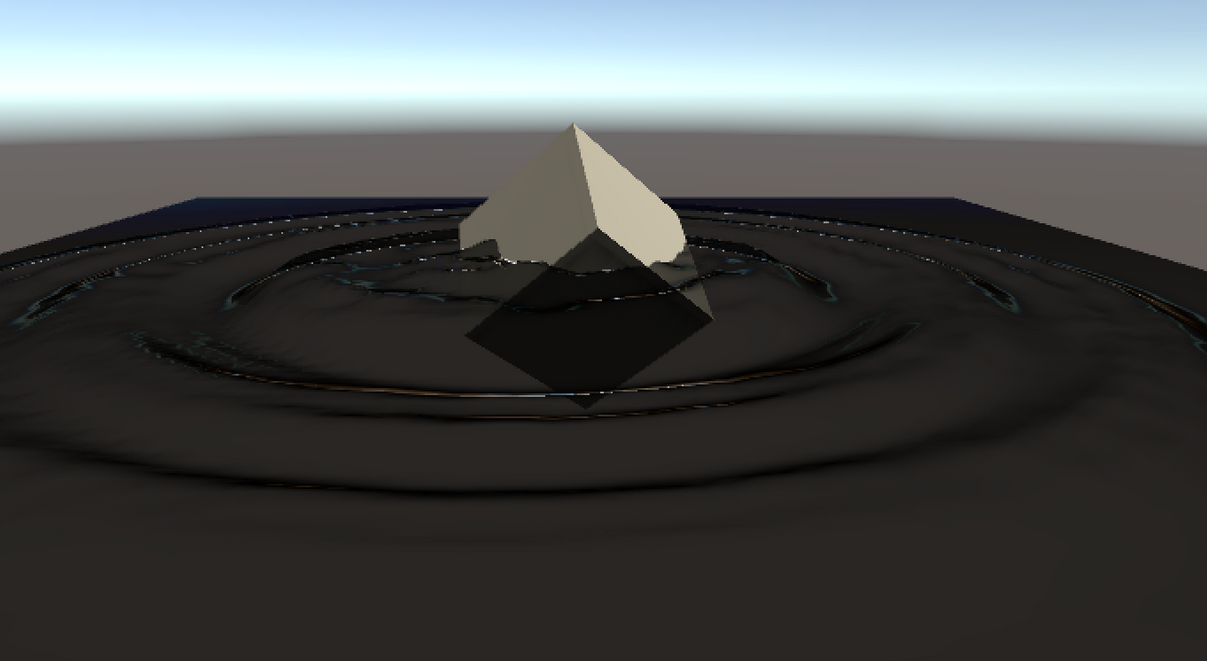
\includegraphics[width=0.8\linewidth]{waveparticles_example}
\caption{The output of wave particles system \cite{WaveParticlesGPU}.}
\label{fig:waveparticles_example}
\end{figure}

There has been research into pushing forward the state-of-the-art in developing
code for GPUs in more programmer-friendly ways. However, as covered in Chapter
\ref{chp:related_work}, much of the research has either been domain-specific or
provided abstractions which have an unacceptable performance overhead for many
use-cases \cite{TODO}. For example, a common approach is to design a unified
language which can be compiled to a run-time that supports GPUs, as is the case
with Lime and Halide \cite{Lime2010} \cite{Halide}. However, by hiding the
details of the heterogeneous backends it targets, Lime has no facility for
allowing the programmer to control how data is transferred between various
components, something which is crucial in game development \cite{TODO}. Working
with low-level toolchains is an odd mix of using an API and writing code in a
GPU-specific language such as GLSL or HLSL. Research has primarily focused on
hiding the API and simplifying GPU-specific elements by designing unified
languages to abstract those details. We demonstrate that alternative approaches
which improve aspects of low-level toolchains exist.

We provided the motivation for the solutions described in this paper, first by
explaining the prevalence of GPUs and how important improvements to toolchains
which target them could be. Secondly, we demonstrated the problems low-level
toolchains face using a water simulator as brief example. Finally, we provided
a brief explanation of why research has yet to tackle these problems.

\section{The Solutions}

\label{sec:solutions_introduction}

We introduce our two systems, AnnoCheck and CUG, which we present as solutions
to the problems described above. First we describe what the desired outcomes of
those solutions should be and how they should improve over the status quo. We
then introduce the solutions themselves; firstly describing the annotation
processor AnnoCheck, before explaining its limitations. This led us to develop
CUG: a programming language with two distinct dialects.

\subsection{Desired Outcome}

As we describe in Chapter \ref{chp:related_work}, systems which aim to improve
over low-level toolchains often sacrifice some control that those traditional
workflows provide: whether it be memory management, scheduling, or which
hardware sections of code eventually target. This has two benefits: improving
the user-experience by abstracting-away low-level details, and providing an
optimising compiler with the control necessary to optimise scheduling. The
issue with this approach is the fact that precise control is still important in
many domains where GPUs are used -- to the point where programmers still choose
to make the trade-off of working directly with APIs like OpenGL or Vulkan
\cite{TODO}. Therefore, solutions which aim to build and improve upon the
status quo should provide all the options that traditional toolchains offer,
including exposing any underlying GPU APIs.

Although this means these solutions are limited in the abstractions that they
can provide, there are some ``easy wins'' to be made. This is demonstrated by
the example problem shown in Listing \ref{lst:c_sharp_hlsl_struct_comparison}
and elaborated on in Section \ref{sec:api_challanges}. Some bugs introduced due
to errors in using a GPU API can be prevented by compile-time checks. That is,
instead of trying to unify code that is written for the CPU and GPU under a
single language or system which is designed to generate API calls for the
programmer, we can use compile-time checking \textit{between} CPU and GPU
languages in order to catch errors which would otherwise be left undetected.

In conclusion, any solution that aims to improve upon current programming
models should deliver the benefits described above without sacrificing anything
low-level toolchains provide. This can be done by targeting specific classes of
errors as described in Section \ref{sec:api_challanges}. We can do this with
two techniques: compile-time cross-language checks and the processing of
annotations to check the validity of raw API calls.

\subsection{What was done}

We created two prototype systems for checking programs across language
boundaries in CPU-GPU systems. Both demonstrate a different approach in
implementing compile-time cross-language checks and checking the validity of
raw API calls for graphics programming. We chose to target the Vulkan API to
demonstrate that these ideas can work at the very lowest-level. However, the
ideas are also applicable to other APIs such as OpenGL, or Direct3D.

We first developed \textit{AnnoCheck}, a pre-processor for C and GLSL that
operates on annotated sections of code. The goal here was to demonstrate how an
existing pair of languages with similar type systems could be extended in order
to have error-checking on raw API calls. Furthermore, as C and GLSL are a
common language pairing for graphics programming, a lot of existing code could
stand to benefit from these techniques \cite{TODO}. We chose C and GLSL as they
share enough similar \textit{syntactic} properties to already allow the
programmer to share some code between them (such as struct definitions).
Although this approach has the benefit of being able to \textit{plug-in} to
existing C and GLSL code, it does have some limitations. Firstly, the sharing
of code is limited to a syntactic happenstance without guarantees, which could
result in errors (Section \ref{sec:api_challanges}). Secondly, C's type system
has limitations compared with many modern languages. As we discuss in Chapter
\ref{chp:conclusion_and_further_work}, there are many opportunities presented
by sharing code \textit{semantically} instead of just \textit{syntactically}.

% TODO(Image!): include diagram of all the wokflows?

This led us to develop the \textit{CUG} compiler, which can compile two
language \textit{dialects} called CUG-C and CUG-G. The first goal was to
demonstrate the power that the semantic sharing of code could provide in
solving the problems we describe in Section \ref{sec:api_challanges}, as these
two dialects share the same compiler. The second goal was to show how existing
high-level languages could be extended with a shader-language. This would be
suitable for a language such as C$^\sharp$, which has a strong type system, but
is compromised and arguably \textit{less safe} than C when using shaders, as it
cannot share any code with them as shown in Listing
\ref{lst:c_sharp_hlsl_struct_comparison}. Due to resource limitations, we
designed CUG-C and CUG-G from scratch with the minimum subset of features
required in order to demonstrate that this is possible, instead of extending an
existing full-featured language such as $C^\sharp$.

One thing to note is that our goal was not to write a comprehensive set of
tools which could be used to catch all errors of this nature at compile-time.
We instead hope to show some ideas which could be used to catch various kinds
of errors, by demonstrating implementations of two prototype systems which have
been designed to capture a small subset of them. Although limited, both
projects came to a total of over 13,000 lines of code, excluding whitespace,
comments, or any example programs that we use to test these two systems.

\subsection{AnnoCheck}

AnnoCheck is a command-line program that takes annotated code written in C and
GLSL as input. An example annotation and the code that is generated is shown in
Listings \ref{lst:annotation_example_input} and
\ref{lst:annotation_example_output}. These are small snippets of the larger
program used in our Evaluation (Chapter \ref{chp:evluation}), adapted from an
example program written by Neil Henning \cite{VulkanComputeExampleSource}
\cite{VulkanComputeExampleBlog}.

\begin{lstfloat}
\begin{center}
Annotated C\footnote{We used designated initialisers in C to make it easer to
read the code \cite{DesignatedInitC}.}
\end{center}
\begin{lstlisting}[language=C]
VkComputePipelineCreateInfo compute_pipeline_create_info = {
    .sType = VK_STRUCTURE_TYPE_COMPUTE_PIPELINE_CREATE_INFO,
    // The @create_verification command is processed by
    // AnnoCheck and converted into C.
    .stage = @create_verification(
        struct: VkComputePipelineCreateInfo,
        // "verification_1" is the name of the annotation
        name: "verification_1",
        data: {
            .sType = VK_STRUCTURE_TYPE_PIPELINE_SHADER_STAGE_CREATE_INFO,
            .stage = VK_SHADER_STAGE_COMPUTE_BIT,
            .module = shader_module,
            // the struct references the main function below
            .pName = "main"
        }
    ),
    .layout = pipeline_layout
};
VkPipeline pipeline;
vkCreateComputePipelines(
    vulkan_device, 0, 1, &compute_pipeline_create_info,
    0, &pipeline
);
\end{lstlisting}
\begin{center} Annotated GLSL \end{center}
\begin{lstlisting}[language=C]
// The shader is verified against "verification_1"
@verify(from: "verification_1", function:
void main() {
    output_buffer.values[gl_GlobalInvocationID.x] = input_buffer.values[gl_GlobalInvocationID.x];
})
\end{lstlisting}
\caption{Annotated C and GLSL that can be processed by AnnoCheck. The output
that AnnoCheck produces for these snippets is shown in
Listing \ref{lst:annotation_example_output}. The full example can be found on
the project GitHub repository \cite{ProjectSource}.}
\label{lst:annotation_example_input}
\end{lstfloat}

As we will describe, Listing \ref{lst:annotation_example_input} shows an
example of an API call that can result in an error that could be checked-for at
compile-time. Here, the host code makes the \texttt{vkCreateComputePipelines}
API call in order to create a compute pipeline\footnote{This is just an API
call that needs to be made in order to run a non-graphics (compute) shader on
the GPU \cite{TODO}.} \cite{vkCreateComputePipelines}. An instance of the
\texttt{VkComputePipelineCreateInfo} struct containing a
\texttt{VkPipelineShaderStageCreateInfo} struct is passed to that API call,
which ultimately specifies which function in the shader to use within the
compute pipeline \cite{VkComputePipelineCreateInfo}
\cite{VkPipelineShaderStageCreateInfo}. Annotations are used to label the
creation of the \texttt{VkPipelineShaderStageCreateInfo} structure on the host
and the \texttt{main} function within the shader using the
\texttt{@create\_verification} and \texttt{@verify} commands respectively. The
annotation itself is given a name, \texttt{"verification\_1"}, which the
annotated C and GLSL reference. AnnoCheck takes annotated code as input and
produces the output seen in Listing \ref{lst:annotation_example_output}.

\begin{lstfloat}
\begin{center} Output C \end{center}
\begin{lstlisting}[language=C]
VkComputePipelineCreateInfo compute_pipeline_create_info = {
    .sType = VK_STRUCTURE_TYPE_COMPUTE_PIPELINE_CREATE_INFO,
    .stage = {
        .sType = VK_STRUCTURE_TYPE_PIPELINE_SHADER_STAGE_CREATE_INFO,
        .stage = VK_SHADER_STAGE_COMPUTE_BIT,
        .module = shader_module,
        .pName = "main",
    },
    .layout = pipeline_layout,
};
VkPipeline pipeline;
vkCreateComputePipelines(
    vulkan_device, 0, 1, &compute_pipeline_create_info,
    0, &pipeline
);
\end{lstlisting}
\begin{center} Output GLSL \end{center}
\begin{lstlisting}[language=C]
void main()
{
    output_buffer.values[gl_GlobalInvocationID.x] = input_buffer.values[gl_GlobalInvocationID.x];
}
\end{lstlisting}
\caption{The output generated from Listing \ref{lst:annotation_example_input}
by AnnoCheck. The full example can be found on the project GitHub repository
\cite{ProjectSource}.}
\label{lst:annotation_example_output}
\end{lstfloat}

% @Old
% The annotation provides two key features in this particular example. The first
% is the generation of boiler-plate for the creation of the
% \texttt{VkPipelineShaderStageCreateInfo} struct. This was done to investigate
% boiler-plate generation features a pre-processor could provide. The second and

The important key feature this example provides is the compile-time checking of
the function name -- ensuring that \texttt{main} cannot be renamed in the host
or shader without being consistently renamed in the other. If we deliberately
introduced such an error was into raw C and GLSL, the resulting behaviour would
be a runtime crash. However, not all such inconsistencies result in runtime
errors, others can simply result in incorrect or undefined runtime results
(Appendix \ref{app:other_API_issues}).

Listing \ref{lst:annotation_example_input} demonstrates how annotations can
prevent programmers from compiling code where the names of shaders differ
between C and GLSL, informing them of the runtime error that this would cause.
The flexibility of AnnoCheck is that the programmer can remove the annotations
if they desire, especially when using complex runtime features. However,
AnnoCheck can still help ensure that an initial implementation is correct.
Furthermore, Section \ref{sec:design_annotation_processor} covers design
decisions that were made with typical shader workflows in mind such that
annotations can be kept for most use-cases.

\subsection{CUG}

CUG consists of two \textit{separate} but \textit{semantically related}
languages called \textit{CUG-C} and \textit{CUG-G}, each designed to target
different architectures. However, due to them being semantically related, we
refer to them as \textbf{dialects}. The first dialect, \textit{CUG-C}, is
designed to be compiled for the CPU. The second dialect, \textit{CUG-G} is
similarly designed to target GPUs.

% Section \ref{sec:TODO} explains how historically compiling custom languages to
% shaders has been a difficult endeavour, due to a plethora of inconsistencies
% between the implementation of shader languages by different GPU vendors. The
% recent development of intermediate shader languages mitigate this problem,
% allowing custom shader languages to be developed \cite{TODO}. TODO(Content): is this really needed?

We demonstrate a prototype system that allows programmers to write host-code
and shaders in programming languages that have modern features, without
sacrificing the low-level control that C and GLSL provide. We additionally
demonstrate the power that semantically sharing code can provide, compared with
the syntactic sharing of code that typically happens between C and GLSL.
Similar to how different natural-language dialects have mutually-intelligible
subsets, CUG-C and CUG-G have a mutually intelligible subset called CUG-min
that allows them to share code \textit{modules} (files).

% TODO(Content): Find a suitable place to mention how non-nullable pointers can
% enrich an existing graphics API.

% TODO(Task): Read https://www.khronos.org/registry/spir-v/specs/1.0/SPIRV.pdf

\begin{lstfloat}
\begin{center} CUG-C \end{center}
\begin{lstlisting}[language=C]
let shader_interface :Shader_Interface = @define_shader_interface(name="main");
let compute_pipeline_create_info: [] C::VkComputePipelineCreateInfo = [{
    sType = VK_STRUCTURE_TYPE_COMPUTE_PIPELINE_CREATE_INFO,
    pNext = null,
    flags = 0,
    stage = get_VkPipelineShaderStageCreateInfo(
        shader_interface=shader_interface
    ),
    layout = pipeline_layout,
    basePipelineHandle = 0,
    basePipelineIndex = 0
}];
var pipeline : C::VkPipeline;
C::vkCreateComputePipelines(
    device=vulkan_device,
    pipelineCache=0, createInfoCount=length(compute_pipeline_create_info),
    pCreateInfos=get_c_ptr_from_array(compute_pipeline_create_info),
    pAllocator=null,
    pPipelines=&pipeline
);
\end{lstlisting}
\begin{center} CUG-G \end{center}
\begin{lstlisting}[language=C]
let main() {
    output_buffer.values[gl_GlobalInvocationID.x] =
        input_buffer.values[gl_GlobalInvocationID.x];
}
\end{lstlisting}
\caption{Code written in CUG-C and CUG-G that has the same functionality as
Listing \ref{lst:annotation_example_input}. The full example can be found on
the project GitHub repository \cite{ProjectSource}. The Syntax is given in
\ref{sec:language_syntax}.}
\label{lst:language_example}
\end{lstfloat}

Listing \ref{lst:language_example} shows a snippet of code with the same
functionality as the annotation example shown in Listing
\ref{lst:annotation_example_input}. As can be seen, CUG-C has an in-built
directive system similar to the annotation system we created for C and GLSL.
This is used to tell the CUG compiler about the existence of a shader interface
with the name ``main''. The compiler can then check for conformance of that
interface when compiling CUG-G. We are not advocating for any particular
features of these dialects, but rather demonstrate some of the benefits a
multi-dialect system can provide. We also explore the opportunities such a
system presents in Chapter \ref{chp:conclusion_and_further_work}.

The syntax, semantics and particular features of these languages are provided
in-depth in Section \ref{sec:design_languages}. Due to the verbose nature of
using GPU APIs, further CUG examples are given in Appendix
\ref{app:other_cug_examples}.

\section{Summary}

We have presented AnnoCheck and CUG, giving the motivation their creation. We
have explained that despite the existence of many techniques which
abstract-away GPU APIs, therefore simplifying heterogeneous programming,
traditional toolchains will still be used in many contexts for the forseeable
future. However, this does not mean that those traditional toolchains cannot
themselves be improved. Our first attempt, AnnoCheck, is designed to allow
programmers to annotate C and GLSL code in order to provide limited
cross-language checking. However, due to limitations with this approach, we
developed CUG, a multi-dialect programming language that solves some of the
problems we experienced with AnnoCheck. However, both systems have merits, and we
demonstrated some examples where they can help prevent common errors when using
GPU APIs.

\chapter{Technical Background}

\label{chp:technical_background}

We summarise the relevant history of graphics hardware and how it developed
over time to become useful in many fields beyond real-time rendering in video
games. Following that, the evolution of graphics APIs is provided, to give both
the context for the problem this paper aims to tackle and the underlying
technology the solutions depend upon. We explain how the complexities of
competing programming models for GPU programming, and therefore how the lack of
an ``hourglass'' ecosystem has limited the development of GPU-targeted
languages. Finally, the difficulties and issues with programming for GPUs are
summarised from the contents of this chapter.

% TODO(Citation): Why low level details are important (eg unified memory versus seperate
% memory)
% https://www.slideshare.net/zlatan4177/gpgpu-algorithms-in-games
% https://en.wikipedia.org/wiki/Heterogeneous_System_Architecture


\section{A (brief) History of GPU computing}

\label{sec:history_gpu}

Graphics Processing Units (GPUs) were originally fixed-function hardware
accelerators for 3D rendering aimed at hobbyist gamers who wanted to play games
with complex graphics \cite{GLQuake}. Due to rapid developments and
competition, the scope and capabilities of graphics cards has expanded such
that they are the highly-parallel general computation machines we find them to
be today. However, the developments GPUs experienced were not pre-planned, and
despite their current general-purpose nature, the terminology surrounding
graphics cards has its foundation in graphics, and is disconnected from
programming language norms. Furthermore, standards around using GPUs and
heterogeneous hardware are still solidifying, with many fragmented communities
and confusion around the future roadmap of GPU APIs \cite{TODO}.

This section summarises relevant milestones related to the history of
heterogeneous computing in order to help the reader understand why the field is
is in a fragmented state that has hindered the development of new shading
languages. Furthermore, by giving context to development of the terms and
technologies used by both of the systems we describe, it provides the relevant
background needed to understand AnnoCheck and CUG.

\begin{itemize}

    \item 1992 \textbf{OpenGL 1.0} released by Silicon Graphics and derived
    from the proprietary ``IrisGL''. Created as an open-standard API for
    interacting with graphics hardware on 3D graphics workstations. The API
    allowed users to issue basic commands in order to set-up 3D scenes, apply
    basic fixed-function lighting, and then render the scenes
    \cite{OpenGL_1_0}. The OpenGL specification is now controlled by the
    \textbf{Khronos Group} \cite{OpenGL} \cite{OpenGLToKhronos}.

    \item 1996 \textbf{Direct3D 2.0} released by Microsoft. Although at this
    point API was designed as an abstraction for a software renderer, it
    eventually developed into an API for interfacing with graphics cards
    \cite{JohnCarmackPlanDirect3DvsOpenGl}.

    % \item 1996 \textbf{3Dfx Voodoo1} graphics card released. Although not the
    % first graphics card, it dominated the consumer market and brought 3D
    % graphics rendering to the mainstream \cite{Voodoo1}.

    \item 1999 \textbf{NVIDIA GeForce 256} released; the first video card to be
    marketed as a \textbf{GPU}. It was the first consumer-PC graphics hardware
    to accelerate ``transform and lighting'' operations, allowing them to be
    offloaded from the CPU. The ``transform and lighting'' component of GPUs
    prefigured what would eventually run shaders \cite{GeForce256}.

    \item 2000 \textbf{The Khronos Group} was founded to provide a formal body
    for open standards in 3D graphics. Reflecting the increasing flexibility of
    graphics cards over time, they have come to additionally provide standards
    in virtual and augmented reality, heterogeneous computing, computer vision,
    parallel computing and neural networks \cite{KhronosGroupAbout}.

    \item 2001 \textbf{GPGPU}, \textit{general purpose computations on GPUs},
    are demonstrated by Larson and McAllister. They perform fast matrix
    multiplications by encoding matrices as the inputs and outputs of the
    graphics pipeline to offload calculations to the GPU \cite{MatrixGPU}.
    Subsequent papers then show how GPUs can outperform CPUs for many
    operations that are desirable in scientific computing \cite{CUDAtoOpenCL}
    \cite{Kruger03linearalgebra} \cite{LUGPU} \cite{SparsematrixGPU}.

    \item 2003 \textbf{OpenGL ES}, released by the Khronos Group for embedded
    systems \cite{OpenGLESRelease}. It is currently the most widely deployed 3D
    graphics API in history, being popular on mobile platforms such as Google's
    Android operating system \cite{OpenGLES}.

    \item 2004 \textbf{GLSL (OpenGL Shading Language} introduced into the
    \textbf{OpenGL 2.0} specification \cite{GLSL_1_10}. It was created to tame
    the complexity and proliferation of custom OpenGL extensions with assembly
    languages that customised parts of the fixed-function pipeline. This
    formally replaced parts of the graphics pipeline with user-programmable
    stages which were defined using a hardware-independent high-level language.
    GLSL at this point was defined as \textit{two} closely-related shading
    languages for different parts of the pipeline: the vertex processor (for
    transforming vertices) and the fragment processor (for operating on
    individual pixels in the final image). GPU vendors are responsible for
    including their own GLSL compilers in their hardware drivers \cite{TODO}.

    \item 2005 \textbf{Unified Shader Architecture} introduced in ATI's
    \textbf{Xenos GPU}, released as part of the Xbox 360. The ``vertex'' and
    ``pixel'' segments of the GPU pipeline are unified into a single component
    that can run either of these. This brought GPUs away from being direct
    fixed-function hardware implementations of the graphics pipeline
    represented by OpenGL and closer to being general-purpose computation
    machines \cite{XenosDemystified}. All GPUs would soon adopt this
    architecture \cite{HistoryOfTheGPU}.

    \item 2006 \textbf{CUDA} (Compute Unified Device Architecture) introduced
    by NVIDIA as a proprietary parallel computation platform and API. This
    allowed programmers to exploit the GPGPU capabilities of graphics hardware
    directly, without having to encode data as the input and output of the
    OpenGL pipeline. This made GPU computing more efficient and accessible
    \cite{AboutCUDA}. \textbf{OpenCL} is a similar open platform created by
    Apple and now maintained by the Khronos Group \cite{OpenCL}.

    \item 2015 \textbf{SPIR-V} shading language released alongside
    \textbf{OpenCL 2.1} \cite{SPIRVLaunch}. Unlike the high-level
    \textit{OpenCL C} and \textit{GLSL} shading languages which drivers need to
    compile themselves, this is an intermediate language based on \textit{LLVM
    IR} which compilers for any language can target \cite{LLVMIR} \cite{SPIRV}.
    SPIR-V support was then added to \textbf{OpenGL 4.6} and supported by
    Vulkan at launch, unifying the shading languages of Khronos' APIs
    \cite{SPIRVOpenGL}.

    \item 2016 \textbf{Vulkan} released by the Khronos Group. A low-level GPU
    API that aims to better represent how modern graphics cards are designed.
    This differs from OpenGL, whose abstraction of a traditional graphics
    pipeline no longer represents the unified nature of GPUs
    \cite{VulkanAnnouncement}. Unlike OpenGL and OpenGL ES, Vulkan is the same
    on desktop, mobile and embedded systems \cite{Vulkan}.

\end{itemize}

\begin{figure}[h]
\centering
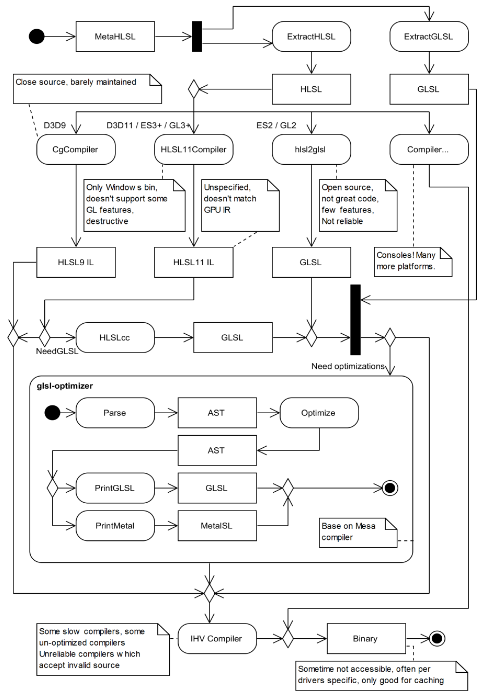
\includegraphics[width=0.6\linewidth]{unity_shader_madness}
\caption{The current state of the Unity game engine shader pipeline
\cite{UnityShaderPipeline}. The complexity comes from the fragmented nature
of GPU APIs.}
\label{fig:unity_shader_madness}
\end{figure}

\begin{figure}[h]
\centering
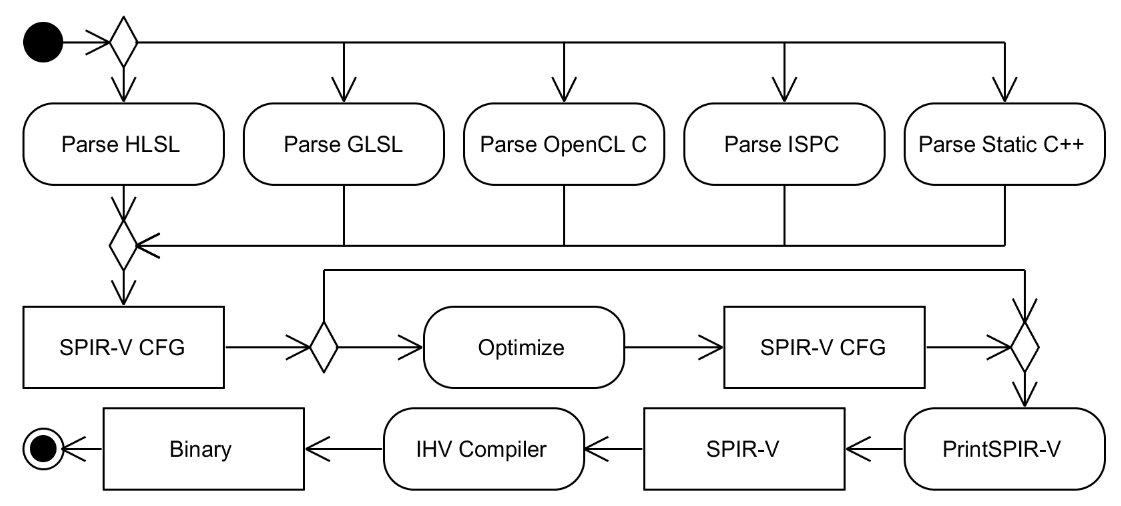
\includegraphics[width=0.8\linewidth]{unity_shader_sanity}
\caption{This is what the Unity shader pipeline shown in Figure
\ref{fig:unity_shader_madness} could look like if SPIR-V becomes the standard
intermediate representation for shader languages \cite{UnityShaderPipeline}.}
\label{fig:unity_shader_sanity}
\end{figure}

The capabilities of GPUs and their related APIs have massively expanded since
they were both introduced, allowing GPUs to be used in increasingly general
domains (Section \ref{sec:motivation}). Unfortunately, as a result of a complex
history, there are many different APIs for different use-cases of the same
hardware (eg. OpenGL vs OpenCL). Furthermore, many of these use-cases have
widely-used proprietary alternatives such as CUDA, Direct3D,
Metal\footnote{Apple's proprietary API.} and even proprietary game console APIs
\cite{CUDA} \cite{Metal} \cite{Direct3D} \cite{PS4PortCrew} (full comparison in
Appendix \ref{sec:api_options}). This makes programming for GPUs in a portable
manner extremely complex. This is shown in Figure
\ref{fig:unity_shader_madness}, which displays how the popular Unity game
engine targets many platforms \cite{UnityShaderPipeline}.

However, with the release of SPIR-V, aspects of the various Khronos Standards
(OpenCL, OpenGL and Vulkan) are converging. Additionally, despite a foundation
in graphics, the compute capabilities of Vulkan are expanding such that OpenCL
could eventually be merged into the API \cite{VulkanOpenCLMerge}. Furthermore,
the low-level nature of new graphics and compute APIs such a Vulkan, Metal and
Direct3D 12 have allowed portability initiatives to bring implementations of
those APIs as light shims above the others \cite{VulkanPortabilityInitiative}
\cite{VulkanPortabilityInitiativeAnnouncement}. Figure
\ref{fig:unity_shader_sanity} shows how the Unity game engine's toolchain could
be simplified using SPIR-V as a backend \cite{UnityShaderPipeline}. This is
much closer to the ``hourglass'' model that CPUs provide, and will hopefully
spur the development of many new shading languages.

\section{The Challenges with the APIs}

\label{sec:api_challanges}

% TODO(Content) mention how Vulkan is merging the OpenGL, OpenCL and OpenGL ES.

% TODO(Helpful): Good comparison of mess vs potential future (Unity Pipeline).
% http://www.g-truc.net/doc/2015%20-%20EuroLLVM%20-%20SPIR-V.pdf
% can also be shown in conclusion.

Due to the complex development history of GPU APIs such as OpenGL (Section
\ref{sec:history_gpu}), they have naturally evolved various issues, mainly as
they reflect how GPUs have \textit{historically} operated \cite{TODO}. However,
this situation has recently improved with the creation of the Vulkan API. This
section does not enumerate all of the issues graphics APIs have, but instead
will briefly describe the workflow and toolchains of using a GPU API, and then
enumerate the challenges our systems aim to ease.

A comprehensive overview of the challenges GPU APIs present are given in
Appendix \ref{app:other_API_issues}.

\subsection{An overview of a typical GPU API}

\label{sec:graphics_api_overview}

A GPU API typically consists of two components: the API itself and a ``shader''
language that is used to write programs that run on the GPU itself. The API
will typically come in the form of a C library, with functions that the user
can call in order to direct an abstracted model of the GPU to perform specific
operations. Some of those API calls enable the user to load their shaders onto
the GPU, transfer data to the GPU, and then execute the shaders on that data.

For graphics operations, the full set of operations needed in order to render
an image is called the \textit{graphics pipeline}
\cite{TripThroughGraphicsPipeline1}. Although there were originally two stages,
modern graphics APIs now expose up to seven shading stages
\cite{TripThroughGraphicsPipeline3}:

\begin{itemize}

    \item \textbf{VS (Vertex Shader)}: Transform vertices.

    \item \textbf{HS (Hull Shader)}: Accept patch primitives and modify patch
    control points.

    \item \textbf{DS (Domain Shader)}: Take control points from HS and convert
    them into vertices.

    \item \textbf{GS (Geometry Shader)}: Take primitives as input and generate
    new primitives from them.

    \item \textbf{PS (Pixel Shader)}: Get interpolated primitive data for each
    pixel, and output pixel color.

    \item \textbf{CS (Compute Shader)}: Its own, separate pipeline. Takes
    buffers as input and write to buffers as output. This is what is used for
    general purpose computionans (GPGPU). OpenCL and CUDA only provide APIs for
    controlling this part of the pipeline.

\end{itemize}

\begin{figure}[h]
\centering
\def\svgwidth{\linewidth}
\input{images/graphics_pipeline_stages.pdf_tex}
\caption{Different graphics pipeline configurations. Each row represents a
possible configuration of the graphics pipeline
\cite{TripThroughGraphicsPipeline3}.}
\label{fig:graphics_pipeline_stages}
\end{figure}

Figure \ref{fig:graphics_pipeline_stages} shows how these stages fit into the
overall graphics pipeline, in addition to showing different configurations of
the pipeline itself. Pipeline 1 shows how the graphics pipeline previously
operated, with only vertex and pixel shading stages. Pipeline 2 shows how the
geometry shader was added, and pipeline 3 shows the addition of the hull and
domain shaders. Pipeline 4 represents the (relatively simple) compute shading
pipeline.

Although conceptually simple, controlling the graphics pipeline is complex. As
we discuss in Chapter \ref{chp:implementation}, we focus on targeting the
compute shading stage of the pipeline through the use of the Vulkan API. As
Vulkan operates at a lower level than OpenGL and OpenCL, the API is incredibly
verbose. As we cover in Chapter \ref{chp:evaluation}, the API calls necessary
to run a simple compute shader is over 700 lines long \cite{ProjectSource}!
However, this verbosity is a feature and not a bug\footnote{We discuss the
tradeoffs this decision makes in Chapter
\ref{chp:conclusion_and_further_work}\cite{TODO}.}.

\subsection{The challenges with shading languages}

\label{sec:shading_langauge_challenges}

Historically, most, if not all, shader languages have been heavily based on the
C-programming language (Appendix \ref{sec:api_options}). Furthermore, these
languages have historically been compiled by the \textit{drivers} for GPUs
\cite{TODO}. This has had a few benefits and drawbacks:

Benefits include:

\begin{itemize}

    \item Writing shaders (eg. in GLSL) is relatively straightforward if you
    are familiar with a C-like language.

    \item If C or a similar-enough language is the host language, some code can
    be shared between shaders and host code.

    \item Having a standardised high-level language helps ensure that the same
    shaders will run on hardware from a variety of different vendors.

    \item Since competing languages (eg. GLSL/HLSL) are all based on C, porting
    code from one shader language to another can even be done by simply
    performing ``find and replace'' operations \cite{PS4PortCrew}.

\end{itemize}

Drawbacks include:

\begin{itemize}

    \item High-level language specifications can be ambiguous, which means
    drivers can implement the same standard in incompatible ways \cite{TODO}.

    \item The \textit{driver} for a piece of hardware must include an entire
    compiler for a high-level language.

    \item GPU drivers are proprietary, and can have bugs where semantically
    equivalent programs have different outputs (Figure \ref{fig:glfuzz})
    \cite{GLFuzz}.

    \item Shaders themselves must be tokenised, parsed, type-checked, compiled
    and optimised at run-time \cite{TODO}.

    \item If the host-language has enough syntactic differences from the shader
    language, data-structures must be defined in both languages (Listing
    \ref{lst:c_sharp_hlsl_struct_comparison}). Furthermore, there are no
    built-in mechanisms to ensure these definitions are consistent -- even at
    run-time.

    \item The C type system is limited compared with more modern programming
    languages.

    \item C and shading languages do have subtle differences. For example the
    \textbf{\texttt{int}} keyword in GLSL specifically defines a 32-bit two's
    complement integer, compared with C, where an \texttt{int} must have at
    least 16 bits and can use various encodings \cite{TODO}. Additionally, the
    placement of the \texttt{const} keyword varies in subtly different ways
    \cite{TODO}. Finally, shading languages natively support intrinsic types
    such as vectors, which many CPU languages do not \cite{TODO}. Therefore
    code sharing does not provide guarantees, and can still be fiddly.

    \item GLSL does not support \texttt{\#include} directives, so code must be
    shared using a custom solution \cite{TODO}.

    \item The CPU still has to refer to many identifiers within a shader using
    strings at runtime. Therefore renaming identifiers in shaders requires
    programmers to manually identify any relevant strings within their
    application.

    % \item As the drivers have their own optimisation systems, code does need to
    % be tuned in non-portable ways for specific hardware if you want to maximise
    % performance \cite{TODO}.

    % \item Cross-compiling is difficult, as optimisation can depend on specific
    % tweaks and implementations of the same shading language can be
    % incompatible. This means that it has been difficult to develop shading
    % languages with semantics and syntax similar to non-C-like languages
    % \cite{TODO}.

    % \item TODO: GLSL can't use \#include, and ints could be defined differently
    % anyway.

\end{itemize}

\begin{figure}[h]
\begin{center}
GLFuzz Bug
\end{center}
\centering

\includegraphics[width=0.8\linewidth]{glfuzz}
\caption{An automated testing framework (GLFuzz) found many bugs in graphics drivers,
which resulted in errors like these. Here, a simple shader was broken by
injecting dead flow-control \cite{GLFuzz}.}
\label{fig:glfuzz}
\end{figure}

% These problems still exist, however, the keys to potentially solving many of
% them are appearing. The first step towards this is the creation of the SPIR-V
% intermediate language \cite{SPIRV}. This is a language that has been designed
% to better represent the low-level instructions GPUs actually use. Therefore,
% drivers need to simply translate these instructions, as opposed to compiling a
% high-level language. The goal here is to reduce the number of implementation
% bugs that have previously occurred \cite{TODO}. Additionally, reference
% language \textit{specifications} can be replaced by a reference language
% \textit{compiler}, which can be open-source and therefore receive input from
% many more individuals. Additionally, the same front-end is now used regardless
% of which hardware code will eventually be compiled for, resulting in much more
% consistent behaviour. As the behaviour of the intermediate language itself is
% more consistent on different platforms configurations, it can be targetted by
% different languages with more stability. An optimiser of the intermediate
% language itself can also be shared.

% The reference compiler has also enabled the creation of more-complex shading
% languages, such as the creation of \textit{OpenCL C++}, which would have been
% much harder to create if each hardware vendor had to write their own compilers
% for this language within their drivers. This is a shader language based on C++
% that allows programmers to use many of C++'s features. Therefore more code can
% be shared between the host and shader, in addition to the advanced type
% checking features C++ provides over C.

As we discussed in Section (\ref{sec:history_gpu}), high-level shading
languages such as GLSL are being phased-out in favour of lower-level
\textit{intermediate languages} such as SPIR-V \cite{SPIRV}. Therefore, modern
toolchains allow the programmer to pre-compile GLSL to SPIR-V. We discuss the
developments this has enabled in Chapter \ref{chp:related_work}.

% Additionally, the same compiler can be shared by the \textit{shader language},
% OpenCL C++, and the ``single-source'' heterogeneous computing system known as
% SYCL. SYCL is a way of writing code for heterogeneous hardware within C++, such
% that the compiler then automatically generates the necessary API calls to run
% that code on heterogeneous hardware. This abstracts many aspects of
% heterogeneous computing in order to make programming for GPUs easier, however
% programmers do sacrifice the control they would otherwise have if they wanted
% to achieve optimal performance. However, by having SYCL and OpenCL C++ share
% the same compiler, the SYCL and OpenCL communities can much more easily share
% code, and migrating between these systems is now possible without having to
% re-write all of the code that has been written for heterogeneous hardware.

% Furthermore, this intermediate language is used by OpenGL, OpenCL and Vulkan,
% meaning new shader/shader languages can target a single back-end and be
% compatible with many APIs. Furthermore, the Vulkan portability initiative
% allows developers to run Vulkan on-top-of different APIs on platforms which may
% not natively support Vulkan itself \cite{TODO}. This will hopefully result in
% an ecosystem which much more closely resembles the ``hourglass model'' that
% CPUs enjoy today.
%TODO(Helpful) cite unity presentation slide.

% Cross-compiling between different intermediate languages for different APIs is
% easier than doing the same for high-level languages \cite{TODO}.

Even with this development, GLSL is still the language of choice for graphics
APIs which use SPIR-V, leaving many presented problems unsolved.

% \begin{itemize}

%     \item To demonstrate the possibilities that SPIR-V presents in allowing any
%     high-level language to have its own shading language. This means that the
%     issue demonstrated in Listing \ref{lst:c_sharp_hlsl_struct_comparison}
%     need no-longer exist.

%     \item To demonstrate how a language which is designed with GPUs as a
%     first-class citizen can have a type-system which results in less
%     error-prone programming for the GPU. However, unlike many other
%     such-languages, explicit API calls can still be made, ensuring programmers
%     still have the control they need in order to optimise code how they would
%     like.

% \end{itemize}

% Although \textit{OpenCL C++} has demonstrated some of this, it does have a few
% limitations. The first is that fact that it is only compatible with OpenCL.
% Although the SPIR-V backend is shared by OpenGL, OpenCL and Vulkan, OpenCL is
% the only API which has enjoyed the creation of a high level shader language
% such as OpenCL C++. OpenGL and Vulkan still use GLSL, which is a C-like
% language with the limitations that incurs. This project aims to demonstrate how
% such a language can target graphics APIs as well. C++ does not treat GPUs as
% first-class citizens, therefore OpenCL C++ has to be designed with the existing
% capabilities of C++ in-mind. This project aims to demonstrate features that a
% language could provide if it is aware of the interactions between shader and
% host languages.

\subsection{Issues Summary}

\label{sec:issues_summary}

We enumerate the two specific issues that AnnoCheck and CUG each solve.
Although there is overlap in which problems each system solves, they differ in
their approaches. Concrete examples of these are evaluated in Chapter
\ref{chp:evaluation}.

\begin{itemize}

    \item \textbf{Referring to Identifiers with Strings}: The CPU refers to
    many identifiers within shaders using strings. As the correctness of this
    cannot be checked by a compiler, this makes refactoring code difficult.
    Especially as mis-matches result in programs crashing at
    run-time\footnote{On an Ubuntu 16.04 machine with an NVIDIA GTX 970 GPU.}.
    AnnoCheck solves this problem through the use of programmer-provided
    annotations. CUG does this through compiler directives and an enhanced type
    system.

    \item \textbf{Sharing Code}: Despite being common when using compute
    shaders, sharing data structure definitions and other code can be difficult
    at best and impossible at worst depending on which host-shader language
    combination is being used (Section \ref{sec:shading_langauge_challenges}).
    By allowing code to be shared semantically, CUG can provide guarantees and
    a formalised way of doing this. AnnoCheck does provide basic syntactic
    code-sharing through the use of an \texttt{@include} annotation.

\end{itemize}


%TODO(Rewrite): Clunky

We have presented the technical background to provide the context and knowledge
needed in order to understand the problems AnnoCheck and CUG tackle. This
includes a history of GPU APIs, an overview of the GPU pipeline, and challenges
when using shaders. We rounded off the chapter with the two specific issues our
systems solve.

% \subsubsection{Issue 1: Redefining Datastructures}

% This issue is demonstrated in Listing \ref{lst:c_sharp_hlsl_struct_comparison}
% and is extremely common when writing host code in a language that differs
% significantly from C.

% A common example is wanting to run a shader which takes a buffer of structs as
% input or output. When using C/C++ as the host language, you do not really have
% any problems, because most common shader languages are based on C. Therefore,
% you can define a struct in a \texttt{.h} header file and include it in both
% your shader and host code.

% An issue arises when host code is written in another language that is distinct
% from C. In this case, when using shaders, you have to define the datastructure
% in both the host and the shader language separately. This is what Listing
% \ref{lst:c_sharp_hlsl_struct_comparison} demonstrates.

% Errors can easily occur when these representations of the same datastructure
% differ. For example, given different definitions, if the CPU fills a buffer
% with a given datastructure and then transfers it to the GPU for it to operate
% on, the resulting behaviour will simply be incorrect. Debugging these kind of
% errors is hard, as there are no runtime or compile time checks, so a programmer
% has to locate it by manual inspection.

% Futhermore, this is not a niche error. For example, the Unity game engine uses
% C$^\sharp$ as a scripting language, whilst using HLSL for shaders \cite{TODO}.
% Between April and July 2015, Unity applications from over 170,000 developers
% were installed on mobile hardware alone \cite{UnityByTheNumbers}.

% We hope to demonstrate how this issue could be tackled through the development
% of a pair of custom languages. We aim to demonstrate how a language that differs
% from C can have a shader language derived from it, so that these errors can
% be avoided. For example, going forward, it could be possible to write shaders
% in Unity using a shader language based on C$^\sharp$ instead of one based on C.

% The reason this has not been previously possible, is because of TODO(Content): find
% other sections explaining why and reference them.

% \subsubsection{Issue 2: Refering to shader/shader names using strings}

% This issue is demonstrated in Listing \ref{lst:annotation_example_output}.

% Running a shader consists of multiple steps, the following are important and
% relevant to this problem. Firstly, a shader needs to be written and saved in a
% file. Then, depending on the API, the shader may need to be compiled into an
% intermediary format in order to run on the GPU. Then, when the application is
% running, it performs three important steps. First, it passes a pointer to the
% the shader data to the API, so that it can handle loading the code onto the
% GPU. Second, it identifies which shader (essentially a function) within that
% code should be run. Third, it then makes an API call to run that shader.

% However, this has an issue, and that is that the shader is identified by a
% string, as shown in Listing \ref{lst:annotation_example_output}, and there are
% no compile-time checks between the shader and the host code in order to make
% sure that the host code identifies a shader that actually exists. As there is
% no direct link between the string that the host code uses to identify the
% shader and the name of the shader itself, refactoring and renaming kernels can
% be tricky.

% For example, misnaming the shader in Vulkan, causes a
% \texttt{VK\_ERROR\_INVALID\_SHADER\_NV} error at runtime.

% % https://www.khronos.org/registry/vulkan/specs/1.1-extensions/man/html/vkCreateComputePipelines.html

% % https://www.khronos.org/registry/vulkan/specs/1.1-extensions/man/html/VkResult.html

% The annotation system and the new languages both aim to catch these errors at
% compile-time using different mechanisms.

\chapter{Design}

We discuss the design of AnnoCheck, a novel pre-processing system for C and
GLSL that ensures the enforcement of interfaces between the two languages.
However, limitations in AnnoCheck lead us onto CUG, a novel prototype language
which natively supports the enforcement of CPU-GPU interfaces through the use
of two distinct dialects: CUG-C and CUG-G. We described their use in Section
\ref{sec:solutions_introduction}.

\section{Design Goals}

As we explained in Section \ref{sec:issues_summary}, the ultimate design goal
of AnnoCheck and CUG is to make programming for GPUs less frustrating and error
prone by catching errors. However, we specifically want to balance the
following concerns:

\begin{itemize}

    \item Unlike other systems which do this, we cannot have \textit{any}
    compromises to the control that existing industry standards such as GLSL
    and OpenGL provide, as many programmers still choose to use them for this
    reason (Section \ref{sec:sec:motivation}).

    \item The design AnnoCheck and CUG cannot be restrictive, that is, they
    should not restrict the set of possible programs that can be made relative
    raw C and GLSL.

    \item Existing workflows need to be accounted for. For example, a commonly
    used feature is the ability to \textit{swap} shaders with identical
    interfaces in-and-out at runtime \cite{TODO}.

\end{itemize}

As we elaborate on in Chapter \ref{chp:related_work}, it is these design goals
that have influenced the novel aspects of both AnnoCheck and CUG.

\section{Build Strategy}

Due to the fact that they aim to solve similar problems, both AnnoCheck and the
CUG compiler have a similar build strategy, ensuring that they work with
typical shader workflows and toolchains. We compare these strategies in Section
\ref{sec:toolchain_comparison}.

One of the reasons it is hard to check the consistency between shaders and host
code is the fact that shaders are loaded onto the GPU by the CPU at run-time
using API calls. Systems such as SYCL circumvent this problem by using
``single-source'' programming models - users write their shaders and host-code
in a single file, and the appropriate API calls are generated by the compiler
(Chapter \ref{chp:related_work}) \cite{TODO}. As the compiler controls how code
is loaded-in at run-time, it can ensure that cross-language interactions are
consistent. However, in addition to preventing optimisations that could be made
to the API calls, this system has various other limitations: one of them being
able to swap and load shaders at run-time based on arbitrary logic.

This capability is important for two reasons: the first is in allowing users to
which shaders render their applications at run-time. For example, a game could
have a high-quality shader that implements a realistic lighting model for
rendering, and a low-quality shader that is less realistic, but can run on
weaker hardware. Being able to change these is important for users and
developers who wish to compare the differences. The second reason arbitrary
run-time shader loading is important, is in allowing artists to quickly iterate
shaders themselves. When designing shaders, being able to ``hot-load'' shaders
is very important. If an entire project needed to be re-compiled every time a
shader was modified, that would massively impede productivity, as changes would
take minutes, not milliseconds, to appear on-screen \cite{TODO}.

Therefore, targeting the Vulkan API (Section \ref{sec:backend_choice}), we take
a novel approach in compiling CPU and GPU code separately. However, by
analysing the CPU code, we can generate metadata which is used to check for
possible errors when analysing shaders.

\section{AnnoCheck}

\label{sec:design_annotation_processor}

AnnoCheck is designed to demonstrate how existing graphics workflows using C
and GLSL (or any other C-like shader) can be improved in order to be less
error-prone, without compromising on the control they provide. Furthermore, the
lessons learned from designing and implementing it influenced the design of the
CUG, which provided these benefits natively as described in Section
\ref{sec:design_languages}.

AnnoCheck is specifically designed to make the errors described in Section
\ref{sec:issues_summary} as hard as possible, that is, making it impossible
for there to be a mis-match in the identifiers that are referred to using
strings in C, and the actual identifiers themselves in GLSL (Section
\ref{sec:resolving_identifiers}).

AnnoCheck achieves this by allowing programmers to annotate C and GLSL to mark
their \textit{intent}. Although this system is very flexible, it does have a
few issues. We evaluate all the tradeoffs this choice makes in Chapter
\ref{chp:evaluation}, and how its limitations led to the design of CUG.
However, although only coming in at 1000 lines of code, and being much simpler
than CUG, AnnoCheck does have a few benefits.

\section{CUG Language Design}

\label{sec:design_languages}

We have previously argued the benefits of syntactic and semantic commonality
between host and GPU code; CUG exemplifies this, and we highlight CUG-C's
features next: Firstly, AnnoCheck's features are directly integrated into the
language design. Secondly to show how by being able to \textit{semantically}
share code with a related shading \textit{dialect} (CUG-G), code sharing can be
made much more robust than with C and GLSL. However, our approach differs from
many other custom languages which have aimed to do this. Similar to AnnoCheck,
we are not abstracting-away any API calls. Therefore CUG is theoretically
capable of the same peak-performance as C and GLSL.

Due to resource constraints, CUG does not aim to replicate \textit{all} of the
features that one would expect from an industrial language such a Java, C, C++,
C$^\sharp$, Swift, Rust, etc. Furthermore, we are not advocating for any
particular language feature that CUG implements beyond the novel ideas that ew
presents. CUG is a proof-of-concept that provides bare-minimum feature-set
needed in order to demonstrate the ideas of this paper and it is very much a
toy language. However, this was still a significant undertaking, with the CUG
compiler taking consisting of over \compilerloccount lines of code without
comments or whitespace.

\subsection{Overall Design}

CUG (CPU-Union-GPU) is a novel proof-of-concept programming language which
consists of two different language \textit{dialects}. CUG-C (CUG-CPU), is a
dialect that is designed to target the CPU. Similarly, CUG-G (CUG-GPU), is a
dialect that is designed to target the GPU. Having two distinct dialects means
that the different languages can each have distinct features which make them
more suited for their target hardware, matching the workflow of programming for
GPUs using C and GLSL. For example, CUG-C is capable of using raw pointers,
whereas CUG-G has access to some of GLSL's built-in functions\footnote{such as
normalize,reflect,sin etc.} \cite{GLSLBuiltIn}.

However, unlike C and GLSL, where code (such as struct definitions) can be
shared \textit{syntactically}, CUG supports the \textit{semantic} sharing of
code through a common dialect of CUG-C and CUG-G: CUG-min, the subset of the
two. This means that interactions between the two languages are
\textit{well-defined}, we can guarantee the same identifier for a given types
(eg. \textit{int}), will mean the same thing in both languages: a 32-bit two's
complement integer (unlike C and GLSL, Section \ref{sec:issues_summary}).

\subsection{Syntax}

\label{sec:language_syntax}

This section gives a brief overview of CUG's syntax. Listing
\ref{lst:cug_min_syntax} gives some examples of CUG-min; the syntax and
features that CUG-C and CUG-G share. Listings \ref{lst:cug_c_syntax} and
\ref{lst:cug_g_syntax} similarly provide examples of CUG-C and CUG-G
respectively.

\begin{lstfloat}
\begin{center} CUG-min Syntax \end{center}
\begin{lstlisting}[language=C]
// Import external module
@add module
// 3 being assigned to a newly-declared 32-bit signed integer
var a_variable : s32 = 3;
// 5 being assigned to the existing variable
a_variable = 5;
// 5 being assigned to a 64-bit unsigned constant
let a_constant : u64 = 5;
// type inference, b_constant has type u64 as well
let b_constant := a_constant;
// compile error: constants are immutable!
/* a_constant = 10; */
// A native string datatype
let a_string : string = "Hello, I am a string";
// A struct type-definition
struct A_Struct {
    member_1 : u32;
}
// Declaring a struct variable, members *must* be named
var a_struct_variable : A_Struct = { member_1 = 10 }
// A function definition
let a_fun(a : A_Struct) => A_Struct {
    // arguments are pass-by-value
    return a;
}
// Function call
let a_struct_constant := a_fun
    // Parameters *must* be named when calling a function
    a = a_struct_variable
);
// An enum definition
enum An_Enum {
    A = 0;
    B;    // = 1
    C;    // = 2
    D = -1;
    E;    // = 0
}
// An enum variable
var a_enum_var := An_Enum.A;
// An if-statement and while loop
if a_enum_var == An_Enum.E { // Will be true
    while a_variable < 10 {
        a_variable = a_variable + 1;
    }
}
\end{lstlisting}
\caption{Examples of syntax which is valid in both CUG-C and CUG-G.}
\label{lst:cug_min_syntax}
\end{lstfloat}

\begin{lstfloat}
\begin{center} CUG-C Syntax\end{center}
\begin{lstlisting}[language=C]
// Embed arbitrary C code within the program! Mitigates CUG-C limitations.
@c_environment {
    #include <stdio.h>

    void print_ln(char const * c_str) {
        printf("%s\n", c_str);
    }
}
// Declaring the existence of an external function, it lives in 'C' namespace
@extern let print_ln(c_str: * const C::char)
// Declaring the existence of an external opaque datatype!
@extern opaque_type FILE;
// Declaring the existence of external opaque values
@extern opaque_value SEEK_END: C::int;
@extern opaque_value SEEK_SET: C::int;
@extern let fopen(
    filename: * const C::char,
    mode    : * const C::char
) => ? C::FILE
// Defining a native-wrapper that takes in-language strings
let print_ln(str: string) {
    // Use external functions/values/types with `C::`
    C::print_ln(str=to_c_string(str=str))
}
// This function is the entry-point, akin to 'main' in C.
let start() => s32 {
    print_ln(str="A string"); // Will be printed by printf!
    let a_constant : s32 = 10;
    // a nullable pointer with constant view of target
    let a_nullable_pointer : ? const s32 = null;
    a_nullable_pointer = &a_constant; // address-of, like C
    // 'malloc' operator only available in CUG-C
    let non_nullable_pointer : * s32 = malloc(s32);
    // non_nullable_pointer gets 'freed' at end of current scope
    defer free(non_nullable_pointer);
    // error, as non_nullable_pointer can't have null assigned
    /* non_nullable_pointer = null; */
    // error, as a_nullable_pointer has constant view of target,
    /* non_nullable_pointer = a_nullable_pointer */
    if a_nullable_pointer != null {
        // OK, '!' makes a nullable pointer non-nullable
        *non_nullable_pointer = *!a_nullable_pointer;
    }
    return 0;
}
\end{lstlisting}
\caption{Examples of CUG-C syntax.}
\label{lst:cug_c_syntax}
\end{lstfloat}

\begin{lstfloat}
\begin{center} CUG-G Syntax\end{center}
\begin{lstlisting}[language=C]
// A directive to verify from 'main'
@verify_from main

// Embed arbitrary GLSL code within the program! Mitigates CUG-G limitations.
@glsl_environment {
    #version 450
}

@layout(local_size_x = 1, local_size_y = 1, local_size_z = 1) in;

    // std430 is related to the packing rules
@layout(set=0, binding = 0, std430) buffer _9
{
    values: [16384] vec3;
} input_buffer;

@layout(set=0, binding = 1, std430) buffer _10
{
    values: [16384] vecv3;
} output_buffer;

}
let main()
{
    // Vec3 is available in CUG-min, making struct-sharing easier
    input : vec3 = input_buffer.values[gl_GlobalInvocationID.x];
    // CUG-G has shader functions (`normalize`), CUG-C does not
    // SEE: https://www.khronos.org/registry/OpenGL-Refpages/gl4/index.php
    output_buffer.values[gl_GlobalInvocationID.x] = normalize(input);
}
\end{lstlisting}
\caption{Examples of CUG-G syntax}
\label{lst:cug_g_syntax}
\end{lstfloat}


The syntax for CUG-C and CUG-G are based on C and GLSL respectively, and
similarly differ from each other \cite{MissingInGLSL}. However, they do differ
from those languages in the following ways:

\begin{itemize}

    \item \texttt{let/var name : type = expression;} is how constants/variables
    are declared and assigned a value\footnote{This syntax is inspired by Swift
    \cite{SwiftSyntax}.}. The types of values can also be inferred by leaving
    the ``\texttt{type}'' declaration empty.

    \item Enums are namespaced. Eg. \texttt{let thing := SomeEnum.value;}.

    \item \texttt{@`command`} is the syntax for giving the compiler certain
    commands, such as importing files, generating shader interfaces, and
    declaring the existence of external symbols.

    \item All parameters in structs and function-calls must be explicitly
    assigned\footnote{There is a tradeoff here. On one hand, code-readability
    increases and breaking-changes to function interfaces are less likely to
    result in 'silent' errors. On the other hand, friction is increased when
    writing code. We do not advocate for either approach, but decided on this
    to see how it felt.}.

    \item C and GLSL code can be embedded in CUG-C and CUG-G respectively by
    wrapping it in \texttt{@c\_environment} or \texttt{@glsl\_environment}
    blocks. Similarly, symbols imported from those languages are accessed using
    the \texttt{C::} or \texttt{GLSL::} namespaces.

    \item CUG-C distinguishes \textit{nullable} (pointers which can have null
    assigned to them) and \textit{non-nullable pointers}. This was done to help
    prevent null-pointer dereferencing within graphics API calls. For example,
    many Vulkan API-calls specify which pointer arguments may or may not be
    null, but C's type system has no way of expressing this.

\end{itemize}

There are naturally many syntax and design choices in CUG that we have not
enumerated here due to space limitations. The exhaustive list of design
decisions made which are not directly related to the problem this paper tackles
are given in Appendix \ref{app:cug_design_decisions}.

%TODO(Content): Formal Grammar

\subsection{Semantics}

The semantics of CUG is heavily inspired by C and GLSL, and this is done for
two reasons: Firstly, it simplifies compiling CUG-C and CUG-G to C and GLSL
respectively. Secondly, our goal is to demonstrate how graphics programming can
be made less error-prone without sacrificing any of the control existing
low-level toolchains provide, and this was the simplest way to do that. Even
compiling this bare-minimum was a lot of work: we had to support all of the
language features necessary to interface with the Vulkan API. Due to this, we
limited the scope of which language features would be provided and how much our
semantics differed from C and GLSL. For example, we did not concern ourselves
with proving our type-system was sound or that CUG provided any safety
guarantees. CUG is an experimental language built from the ground-up and should
be treated as such. The upshot of this is that, barring minor syntax changes,
CUG code should be familiar to those who are familiar with C and GLSL. Section
\ref{subsec:limitations} enumerates the limitations of CUG.

\subsection{Limitations}

\label{subsec:limitations}

Being a single language with two dialects, the CUG compiler was a hefty
undertaking with over \compilerloccount lines of code. However, to prevent
feature-creep and project-bloat, we limited the scope of the dialects in the
following ways:

\begin{itemize}

    \item The design of CUG only formalises its abstract syntax, the concrete
    syntax is left underspecified (e.g. no operator precedence).

    \item CUG-C does not support arrays natively. We circumvent this by
    creating arrays in C, and passing a pointer to them into CUG-C.

    \item Although we target C and GLSL as backends for CUG-C and CUG-G, we
    perform very limited name mangling, meaning the programmer has to be
    careful about how symbols are named to ensure that they do not collide with
    any C/GLSL symbols.

    \item Compiler errors which are outside the scope of checking the CPU-GPU
    interface are limited and sometimes broken.

    \item Declarations of external symbols in C/GLSL are not checked. If they are
    incorrect, it can cause weird behaviour.

    \item CUG does not support type-casting, however, we can define external C
    functions which convert from one type to another can call those.

    \item CUG-G does not support the programming of graphics shaders, only
    simple compute shaders. This is reflected in the chosen benchmark.

    \item CUG does not have native floating-point number support.

\end{itemize}

\subsection{C and GLSL interoperability}

In order to provide zero-overhead API calls, the CUG-C must be able to call
directly into C. This also has an additional benefit, in that C libraries can
be leveraged in order to make up for deficiencies in the language itself.

We chose to target target C as the backend for CUG-C. Although an intermediate
language such as LLVM IR would be the optimal choice for a more-developed
language, C was chosen for two reasons: It was easier to do in the time
available, and the output of the CUG compiler can in-turn be included by
C-programs \cite{TODO}. This allows automated tests of language features, by
having C++ call-into code generated by the CUG compiler (Section
\ref{sec:testing}) \cite{AutomatedTestCode} \cite{AutomatedTestOutput}.
Similarly, CUG-G targets GLSL.

The choice of these targets simplified the embedding of C and GLSL with CUG-C
and CUG-G respectively, as described in Section \ref{sec:language_syntax}. This
allowed us to easily include libraries within CUG, and helped compensate for
the limitations our languages had due to their experimental nature.

Too allow embedded code to be accessed, we used an \texttt{@extern} directive
to save the compiler from having to parse that code itself. By requiring the
programmer ensure these were consistent with embedded code, the compiler could
verify that usage of those identifiers was correct. This was purely a time
saving technique to simplify the CUG compiler.


\begin{lstfloat}
\begin{lstlisting}[language=C]
#c_environment {
    #include<stdio.h>
}

@extern let printf(format : * const C::char)

let print_fish() {
    // Note: c_str is a `magic` function that converts
    // in-language strings to c-strings. A mature
    // implementation would have a standard library that
    // provided this feature.
    C::printf(format = c_str(
        str = "fish"
    ));
    return;
}
\end{lstlisting}
\caption{Example of C-interactions. The \texttt{\#c\_environment} keyword is
used to include the \texttt{stdio.h} header. The \texttt{@extern} is used to
mark the existence of the \texttt{printf} function and define its type. As the
language does not support variadic arguments, the full interface cannot be
represented within the language.}
\label{lst:lang_c_interop}
\end{lstfloat}

Listing \ref{lst:lang_c_interop} demonstrates an example of the features used
to interact with C from CUG-G.

% \subsection{Cross-Dialect Interactions}

% TODO(Content!)

\chapter{Implementation}

\label{chp:implementation}

% This chapter may be called something else\ldots but in general
% the idea is that you have one (or a few) ``meat'' chapters which
% describe the work you did in technical detail.

The source code for AnnoCheck and CUG is publicly available and open-source
\cite{ProjectSource}. Although both are written in C++, Python is also used as
a build-system to enable simple cross-platform builds. Both systems were
developed and tested on both Ubuntu 16.04 and Windows 10 operating systems. The
combined source-code for both projects comes to around \totalloccount lines of
code. \compilerloccount of which are for the CUG compiler alone.

%TODO: Furthermore, the design of CUG necessitated comprehensive semantic analysis,

\section{Choice of Backend}

\label{sec:backend_choice}

%TODO(Rewrite): make sure it better explains why the backend was chosen.

We decided to target the Vulkan graphics and compute API in the implementation
of our systems \cite{Vulkan}. Done for the following reasons:

\begin{itemize}

    \item Vulkan is a modern graphics API with runtime safety-features (such as
    validation layers) that other APIs such as OpenGL lack \cite{TODO}. Our
    goal was to demonstrate how even a modern graphics API could suffer from
    the issues described in Section \ref{sec:api_challanges}, and how our
    systems could introduce compile-time checks for these errors.

    \item Vulkan is already being widely used in the gaming industry, so the
    use-cases described here are applicable to a wide audience.
    %TODO(Helpful) : phrase better).

    \item Vulkan is a low-level API. One of the goals of our systems was to
    demonstrate how they have no runtime overhead, this is done by allowing
    users to make Vulkan API-calls directly.

\end{itemize}

\section{AnnoCheck}

\label{sec:anno_check_implemenation}

AnnoCheck takes the form of a commandline program, that can operate
in two modes:

\begin{itemize}

    \item \textbf{Host Mode}: indicated by the \texttt{-h} flag, allows the
    user to provide an annotated C file as input, with two outputs being given.
    The first output is indicated by the \texttt{--out-c} flag, which tells the
    annnotation processor where to output the processed C file. The second
    output is indicated by the \texttt{--out-metadata} flag, which tells the
    annotation processor where to output metadata associated with the
    annotations. This metadata is used to check GLSL files. An example command
    line instruction would be: \texttt{./annotation\_processor -h input.c
    --out-c output.c --out-metadata check.metadata}.

    \item \textbf{Shader Mode}: indicated by the \texttt{-s} flag, allows the
    user to provide annotated GLSL and metadata file as input, with GLSL being
    provided as the output, or an error, if the GLSL and the metadata are
    inconsistent. An example command line instruction would be:
    \texttt{./annotation\_processor -s input.glsl check.metadata --out-glsl
    output.glsl}.

\end{itemize}

Although AnnoCheck seems simple, the intention is for it to be used as a
command-line program that can be used inside a more comprehensive build
systems. We describe such a toolchain in Section \ref{sec:toolchain_comparison}.

AnnoCheck works by looking for custom ``\texttt{@}'' directives within C or
GLSL code. When such a directive is found, it tokenises and parses the relevant
sections of the provided input using a recursive descent parser, creating an
abstract syntax tree.

For annotated C code, the AST is semantically analysed, with a special
dataformat to store metadata which can be used to ensure that GLSL annotations
which are checked later are consistent with the annotated C.

The annotated GLSL code is checked using a similar strategy.

TODO(Content!): flesh this out more WORK OUT HOW MANY WORDS IT WILL TAKE

\section{CUG Compiler Implementation}

The CUG compiler is a much more complex endeavor than AnnoCheck, coming in at
\compilerloccount lines of code. CUG is a single program which is able to
compile code written in three dialects of CUG: CUG-C, CUG-G, and the subset of
the two, CUG-min. Input for the CUG compiler is achieved in a similar manner to
the input into AnnoCheck, with the compilation of CUG-C generating a metadata
output file which needs to be fed as input when analysing CUG-G programs. An
example of this is given in Section \ref{sec:toolchain_comparison}.

\subsection{Compiler Pipeline}

\label{sec:compiler_pipeline}

\begin{figure}[h]
\centering
\def\svgwidth{\linewidth}
\scriptsize{\input{images/cug_compiler_pipeline.pdf_tex}}
\caption{The CUG compiler pipeline. Arrows indicate the flow of data from
input to output. Boxes represent compiler stages.}
\label{fig:cug_compiler_pipeline}
\end{figure}
%TODO: nive tge furst arriw up top to possibly allow larger text.
%TODO(Error!): Fix the typo in 'Generate output' (C in both!)

Figure \ref{fig:cug_compiler_pipeline} shows the CUG compiler, with the
stages handled in the following ways:

\begin{itemize}

    \item \textbf{Set Internal Dialect State}: Depending on whether a CUG-C,
    CUG-G or CUG-min file is being processed, set the internal compiler state
    associated with that file to the appropriate value (Section
    \ref{sec:internal_state_machine}).

    \item \textbf{Tokenise Input}: Perform lexical analysis and tokenise the
    input file. Invalid tokens can result in compilation errors here which are
    reported back to the user. The set of valid tokens depends on dialect state
    associated with a given file. (eg. CUG-C does not support
    \texttt{@glsl\_environment} tokens).

    \item \textbf{Parse Input}: Parse input and generate abstract syntax tree
    of the language. We implemented this using a custom recursive descent
    parser. The dialect state has little affect on parsing as syntax-tree
    generation should be consistent between all the dialects.

    \item \textbf{Parse Imported Modules and Metadata}: Recursively perform the
    ``parse input'' step on imported modules, and metadata that may be imported
    by CUG-G code.

    \item \textbf{Semantically Analyse Imported Modules and Metadata:} Perform
    semantic analysis of imported modules and metadata.

    \item \textbf{Semantic Analyse}: Resolve types and identifiers on the
    program. This step is where most dialect state-specific work is done. Other
    properties are checked-for as well, such as the presence of cycles in
    struct definitions.

    \item \textbf{Generate IR (Intermediate Representation)}: Generate a
    lower-level intermediate representation of the code. This is done in order
    to simplify the process of outputting to C. Our IR consists of a three
    address code system, with quadruples used as the datastructure to represent
    them \cite{TODO}. All frontends share the same IR, however, certain
    quadruples can only be generated for certain backends (eg. pointers and
    malloc are only available in CUG-C). All name-mangling is performed here,
    and all the modules are rolled into a single data structure which contains
    all the IR needed for the final output.

    \item \textbf{Generate Final Output:} Depending on the internal state
    associated with the root file, generate the final C or GLSL output.

\end{itemize}

\subsection{The Internal State Machine}

\label{sec:internal_state_machine}

In order to ensure that CUG-C and CUG-G can share code semantically, code
written in these dialects share the same compiler. This ensures that there are
not any unexpected differences in how the programs are parsed, especially when
sharing modules between the two dialects. This differs massively from C and
GLSL, which do have peculiar differences which means that sharing code can
result in unexpected behaviour (Section \ref{sec:issues_summary}).

We achieve this through the use of an internal state machine within the
compiler, where each module is associated with one of the following states:

\begin{itemize}

    \item \textbf{\texttt{HOST}:} When in the \texttt{HOST} state, the CUG
    compiler ensures that it only compiles code that conforms to the CUG-C
    dialect.

    \item \textbf{\texttt{SHADER}:} When in the \texttt{SHADER} state,
    similarly, only CUG-G code can be compiled.

    \item \textbf{\texttt{SHARED}:} When in the \texttt{SHARED} state, only
    CUG-min is parsed.

\end{itemize}

Originally we were going to have two modes of operation, similar to AnnoCheck
(Section \ref{sec:anno_check_implementation}). However, this was replaced by
a state machine for the following three reasons:

\begin{itemize}

    \item The CUG compiler can transition from the CUG-C or CUG-G state to the
    CUG-min state, when either include a CUG-min module.

    \item Although the CUG-G dialect can only be compiled to compute shaders,
    an industrial compiler like this would need to be extended to supported
    other shader types such as vertex, pixel and geometric shaders. These all
    have subtle differences in permitted operations and behaviour -- extending
    the state machine so that these could be handled would be trivial.

    \item As we discuss in Chapter \ref{chp:related_work}, there has been some
    movement towards ensuring ``single-source'' (where shaders are embedded
    within a C++ program) programs and ``multi-source'' (what we are doing)
    programs use similar semantics, so that code from communites which use each
    can be shared. Theoretically, we could extend the CUG compiler to allows
    programmers to embed CUG-G programs within CUG-C ones.

\end{itemize}

This state is preserved throughout the entire compilation pipeline (Section
\ref{sec:compiler_pipeline}), affecting each of the compilation stages in
different ways. Including code from other source-files (which we call module
imports) is affected by the state machine:

\begin{itemize}

    \item CUG-C files can include both CUG-C and CUG-min files.

    \item CUG-G files can include CUG-G files, CUG-min files and generated
    CUG-C metadata (which is generated when a CUG-C file is compiled, and is
    used to validate the interface of a CUG-G file).

    \item CUG-min files can only include other CUG-min files.

\end{itemize}

%TODO: mention benefit somewhere about CUG-C being able to use GLSL shaders and
% CUG-G being callable from C.

These relationships determine which state transitions are valid, and also are
the mechanism through-which code is shared between CUG-C and CUG-G.

\subsection{Testing}

\ref{sec:testing}

Whilst features in the CUG language were being incrementally developed, it was
important to ensure that existing features where behaving as expected as soon
as possible -- therefore we could ensure that none of the features ever
'regressed'. However, using CUG to test itself would not have been ideal, as
errors within the language could lead to vacuously true results.

To solve this problem, we took advantage of the fact that our CUG-C input was
compiled to C, by using a C++ testing framework to call-into CUG-C functions
and test that the results returned matched what was expected. This feature
proved invaluable, and caught many errors. The biggest difficulty was
working-around the name-mangling the CUG compiler performed, but fortunately it
was predictable and consistent.

This process formed the foundation for an automatic regression-testing system,
which we ran automatically on every commit to the main repository
\cite{ProjectSource} \cite{AutomatedTestCode} \cite{AutomatedTestOutput}.

% \subsection{Interfacing with existing languages}

% TODO(Helpful): reference usage of FNV hash for symbol table. \cite{FNVHash}.


\chapter{Evaluation}

\label{chp:evaluation}

% For any practical projects, you should almost certainly have
% some kind of evaluation, and it's often useful to separate
% this out into its own chapter.

This chapter evaluates how AnnoCheck and CUG compare with the traditional
unchecked C and GLSL toolchain. We do this using a sample program called
\textit{FishCopy}, comparing aspects such as toolchain complexity, code
samples, which errors AnnoCheck and CUG prevent, in addition to analysing how
the resulting code performs. Due to the complexity of using the Vulkan API, we
will present small samples of this program. The full version of
\textit{FishCopy} can be found on the project GitHub repository
\cite{ProjectSource}. For example, the C code which makes the appropriate API
calls to run a simple compute shader that copies items from one file to another
is over 750 lines long. The example is adapted from an open-source sample
program \cite{VulkanComputeExampleSource}.

\section{Fishcopy}

\textit{Fishcopy} consists of a CPU program which performs the necessary work
to invoke a simple compute shader. CPU fills an array with 16384\footnote{This
value was arbitrarily chosen but is a power-of-two, $2^{13}$} values which are
of the type \texttt{Fish}. \texttt{Fish} is a simple struct whose definition is
given in Listing \ref{lst:struct_fish}.

\begin{lstfloat}
\begin{lstlisting}[language=C]
struct Fish{
    int num_eyes;
    int num_fins;
}
\end{lstlisting}
\caption{The \texttt{struct} definition for the \texttt{Fish} type.}
\label{lst:struct_fish}
\end{lstfloat}

% \begin{figure}[h]
% \centering
% \def\svgwidth{0.8\linewidth}
% \input{images/copy_fish.pdf_tex}
% \caption{FishCopy TODO(Content).}
% \label{fig:copy_fish}
% \end{figure}
% TODO(Image!) Workout why this won't compile.

All the values in the array are then assigned a random integer value using the
C library's \texttt{rand()} function \cite{RandRef}. After the array has been
initialised in this way, its contents are then transferred to a buffer on the
GPU. The CPU then invokes a simple compute shader which copies all of its data
across to another buffer. Both buffers are loaded into arrays on the CPU, which
subsequently confirms that they have matching contents.

Although Fishcopy is simple, it serves two purposes: Firstly, to demonstrate
how both CUG and AnnoCheck can catch errors which could easily be made in even
a simple program. Secondly, to show the benefits that CUG can provide over
AnnoCheck.

\section{Shader Comparison}

\label{sec:shader_comparison}

TODO(Content!): COMPARE THE SHADER EXAMPLES IN DEPTH

Listings \ref{lst:glsl_shader}, \ref{lst:anno_check_shader} and
\ref{lst:cug_g_shader}.

\begin{lstfloat}
\begin{center}
FishCopy GLSL Shader
\end{center}
\begin{lstlisting}[language=C]
#version 450
struct Fish {
    int num_eyes; int num_fins;
};
const int BUFFER_LENGTH = 16384;
layout(local_size_x = 1, local_size_y = 1, local_size_z = 1) in;
layout(set=0, binding = 0, std430) buffer _9
{ Fish values[BUFFER_LENGTH]; } input_buffer;
layout(set=0, binding = 1, std430) buffer _10
{ Fish values[BUFFER_LENGTH]; } output_buffer;
void main()
{
    output_buffer.values[gl_GlobalInvocationID.x].num_eyes = input_buffer.values[gl_GlobalInvocationID.x].num_eyes;
    output_buffer.values[gl_GlobalInvocationID.x].num_fins = input_buffer.values[gl_GlobalInvocationID.x].num_fins;
}
\end{lstlisting}
\caption{GLSL version of FishCopy shader. Without helper-tools, the
\texttt{Fish} needs to be manually included in the shader file.}
\label{lst:glsl_shader}
\end{lstfloat}

\begin{lstfloat}
\begin{center}
AnnoChecked FishCopy GLSL Shader
\end{center}
\begin{lstlisting}[language=C]
#version 450
@include "struct.h"
layout(local_size_x = 1, local_size_y = 1, local_size_z = 1) in;
// std430 is related to the packing rules
layout(set=0, binding = 0, std430) buffer _9
{ Fish values[BUFFER_LENGTH]; } input_buffer;
layout(set=0, binding = 1, std430) buffer _10
{ Fish values[BUFFER_LENGTH]; } output_buffer;
@verify(from: "test_shader", function:
void main() {
    output_buffer.values[gl_GlobalInvocationID.x].num_eyes = input_buffer.values[gl_GlobalInvocationID.x].num_eyes;
    output_buffer.values[gl_GlobalInvocationID.x].num_fins = input_buffer.values[gl_GlobalInvocationID.x].num_fins;
})
\end{lstlisting}
\caption{AnnoChecked version of the GLSL FishCopy shader. AnnoCheck provides
the \texttt{@include} annotation for including C structs. However, this does
have its dangers (Section \ref{sec:TODO}). The \texttt{@verify} directive
verifies that the main function conforms to expectations.}
\label{lst:anno_check_shader}
\end{lstfloat}

\begin{lstfloat}
\begin{center}
FishCopy CUG-G Shader
\end{center}
\begin{lstlisting}[language=C]
@add module
// ensures that the interfaces in this module match the one generated by main
@verify_from main
@glsl_environment {
    #version 450
}
@layout(local_size_x = 1, local_size_y = 1, local_size_z = 1) in;
@layout(set=0, binding = 0, std430) buffer _9
{ values: [BUFFER_LENGTH] Fish; } input_buffer;
@layout(set=0, binding = 1, std430) buffer _10
{ values: [BUFFER_LENGTH] Fish; } output_buffer;
let main()
{
    output_buffer.values[gl_GlobalInvocationID.x].num_eyes = input_buffer.values[gl_GlobalInvocationID.x].num_eyes;
    output_buffer.values[gl_GlobalInvocationID.x].num_fins = input_buffer.values[gl_GlobalInvocationID.x].num_fins;
}
\end{lstlisting}
\caption{CUG-G FishCopy shader. Custom directives allow for CUG-min modules to
be included. }
\label{lst:cug_g_shader}
\end{lstfloat}



\section{Toolchain Comparison}

\label{sec:toolchain_comparison}

Figures \ref{fig:pipeline_basic}, \ref{fig:pipeline_anno_check},
\ref{fig:pipeline_cug} and \ref{fig:pipeline_cug_future} compare the build
process of FishCopy for different graphics toolchains. We managed the build
process for all these configurations using a simple Python script.

\begin{figure}[h]
\centering
\def\svgwidth{0.8\linewidth}
\input{images/pipeline_basic.pdf_tex}
\caption{How the C and GLSL version of FishCopy is compiled and run. GLSL lacks
an \texttt{\#include} directive, meaning that programmers need to manually
ensure that shared code is compiled into the shader.}
\label{fig:pipeline_basic}
\end{figure}
%TODO(Error!): Replace 'insert with custom program' with 'manually insert.

Figure \ref{fig:pipeline_basic} shows how the raw C and GLSL versions of
Fishcopy are compiled and executed. In this instance, the \texttt{Fish} struct
is defined in a file called struct.h, which is included in the main program
using C's \texttt{\#include} directive. Although the struct definition is
syntactically valid GLSL as-is, it needs to be manually inserted into the
shader as GLSL does not have a method for including code from other files
\cite{TODO}. This naturally increases the complexity of the "traditional"
toolchain. We compile main.c to an executable using clang, and we compile the
shader to SPIR-V using the Khronos Group's GLSL compiler, glslang \cite{TODO}.

When the executable runs, it performs all the AI calls necessary to load the
compiled SPIR-V shader and execute it on the GPU.

\begin{figure}[h]
\centering
\def\svgwidth{0.8\linewidth}
\input{images/pipeline_annocheck.pdf_tex}
\caption{The AnnoCheck-supported build process for FishCopy. AnnoCheck includes
directives which allow C headers to be inserted into GLSL shaders. However, this
comes with no guarantees about the correctness of doing so.}
\label{fig:pipeline_anno_check}
\end{figure}

Figure \ref{fig:pipeline_anno_check} demonstrates the AnnoCheck version of this
toolchain. As can be seen, there is an extra level of complexity here compared
with the C and GLSL version. The process derived from that for raw C and GLSL,
but with a couple of minor differences. Firstly, AnnoCheck processes the
annotations in main.c in order to generate a metadata file,
\textit{annotations.meta}, that is used to verify the code in the shader. The
second difference is that AnnoCheck is able to perform the same file-inclusion
capabilities for the shader that previously had to be done manually, and whilst
doing so it verifies the shader and, only if the annotations within it are
consistent with main.c, it generates the GLSL shader file.

From this point on, the build process is identical to raw C and GLSL, with the
generated C and GLSL files matching the raw C and GLSL files identically -- the
annotations are simply stripped-out by AnnoCheck after the annotated input
files have been verified.

\begin{figure}[h]
\centering
\def\svgwidth{0.8\linewidth}
\input{images/pipeline_cug.pdf_tex}
\caption{The build process for the CUG version of FishCopy. CUG-C and CUG-G
semantically share the same module. However, compiling to C and GLSL
complicates the build process.}
\label{fig:pipeline_cug}
\end{figure}

Figure \ref{fig:pipeline_cug} demonstrates the CUG toolchain we implemented.
Compared with the simple syntactic sharing of the \texttt{Fish} definition in
both the raw and AnnoCheck toolchains, the module containing \texttt{Fish} is
shared semantically between CUG-C and CUG-G. However, as we describe in Section
Section \ref{sec:backends}, the toolchain complexity is increased by the need
to compile the resulting C and GLSL that is generated by the CUG compiler.

\begin{figure}[h]
\centering
\def\svgwidth{0.8\linewidth}
\input{images/pipeline_cug_future.pdf_tex}
\caption{If the CUG compiler could generate SPIR-V and x86 itself, then the build
process would be simpler.}
\label{fig:pipeline_cug_future}
\end{figure}

Figure \ref{fig:pipeline_cug_future} shows what an idealised CUG toolchain
would look like, that is, if CUG-G was compiled directly to SPIR-V and if CUG-C
was compiled directly to x86.

All the toolchains make different tradeoffs. The raw C and GLSL is the
simplest, but suffers from requiring programmers to use custom solutions for
code-sharing between C and GLSL. Furthermore, interactions between C and GLSL
are completely unchecked -- programmer discipline is what ensures bug or
erroneous behaviour does not occur when making API calls. AnnoCheck increases
the toolchain complexity, in exchange for allowing the programmer to annotate
their code such that AnnoCheck can prevent some errors from happening.
Futhermore, AnnoCheck can also handle code-inclusion in GLSL, removing the need
for that to be done by a custom solution. The CUG compiler is part of the most
complex toolchain, however, this was purely a result of how we implemented the
compiler due to the constraints we faced. Figure \ref{fig:pipeline_cug_future}
demonstrates that if implemented well, a custom language could actually reduce
the overall toolchain complexity, even when compared with raw C and GLSL, by
providing standardised methods for semantically sharing code between host and
shader code (in this case, CUG-C and CUG-G).

\section{Error-Prevention}

In this section we analyse each of the errors shown in Section
\ref{sec:issues_summary}, demonstrating how both the annotation system and
custom heterogeneous languages prevent the programmer from making them.

\subsection{Resolving Identifiers}

\label{sec:resolving_identifiers}

This is an issue solved by both the annotation system and the new set of custom
languages. As we discuss in Section \ref{sec:issues_summary}, host code often
has to refer to identifiers which are mentioned in shaders through the use of
strings. However, this is problematic, for two reasons: Firstly, the
identifiers are not resolved until runtime, when API calls are made by the CPU
that refer to identifiers within a shader that has been loaded onto the GPU.
Secondly, it makes refactoring tools harder to implement, as there is no
logical connection between strings in a host language and identifiers within a
shader that can be statically determined.

This is the primary issue that AnnoCheck aims to resolve, and one of the
features that CUG handles within its cross-dialect type system. Section
\ref{sec:shader_comparison} compares the raw GLSL shader, the annotated GLSL
shader, and the CUG-G shader. Listings \ref{lst:invoke_main_c},
\ref{lst:invoke_main_anno} and \ref{lst:invoke_main_cugc} show how each of
these systems invoke the \texttt{main} function within the shader.

\begin{lstfloat}
\begin{lstlisting}[language=C]
VkPipelineShaderStageCreateInfo shader_stage_create_info = {
  .sType = VK_STRUCTURE_TYPE_PIPELINE_SHADER_STAGE_CREATE_INFO,
  .pNext = 0,
  .flags = 0,
  .stage = VK_SHADER_STAGE_COMPUTE_BIT,
  .module = shader_module,
  .pName = "main",
  .pSpecializationInfo = 0
};
\end{lstlisting}
\caption{The C declaration and initialisation of the datastructure needed to
identify the correct function within the GLSL shader. We use explicit initialisers
in C\cite{TODO}.}
\label{lst:invoke_main_c}
\end{lstfloat}

Listing \ref{lst:invoke_main_c} demonstrates the C implementation of creating a
\texttt{VkPipelineShaderStageCreateInfo} data structure instance. This
structure is what is used by the Vulkan API to identify \texttt{main}, using a
string. This is similar to the example shown in Listing
\ref{lst:annotation_example_output}.

TODO(Content!) On Ubuntu desktop renaming "main" causes a runtime crash, with
no helpful error info. COMPLETE OTHER SECTIONS. DETERMINE WORD COUNT.

\begin{lstfloat}
\begin{lstlisting}[language=C]
VkPipelineShaderStageCreateInfo shader_stage_create_info = @create_verification(
  struct: VkComputePipelineCreateInfo,
  name: "test_shader",
  info: {
    .sType = VK_STRUCTURE_TYPE_PIPELINE_SHADER_STAGE_CREATE_INFO,
    .pNext = 0,
    .flags = 0,
    .stage = VK_SHADER_STAGE_COMPUTE_BIT,
    .module = shader_module,
    .pName = "main",
    .pSpecializationInfo = 0
  }
);
\end{lstlisting}
\caption{The AnnoChecked version of what is shown in Listing
\ref{lst:invoke_main_c}. The struct initialisation is wrapped by an annotation
which is used to ensure that the shader \texttt{main} exists when the
AnnoChecked shader is processed.}
\label{lst:invoke_main_anno}
\end{lstfloat}

\begin{lstfloat}
\begin{lstlisting}[language=C]
let shader_name : ShaderName = @verified_shader_function(main);
let compute_pipeline_create_info :
 C::VkPipelineShaderStageCreateInfo = {
  sType               = VkStructureType.VK_STRUCTURE_TYPE_PIPELINE_SHADER_STAGE_CREATE_INFO,
  pNext               = null,
  flags               = VkPipelineShaderStageCreateFlags.none,
  stage               = VkShaderStageFlagBits.VK_SHADER_STAGE_COMPUTE_BIT,
  module              = shader_module,
  // Below is type-checked thanks to @verified_shader_function
  pName               = shader_name, // entry point of the function
  pSpecializationInfo = null
};
\end{lstlisting}
\caption{The CUG-C initialisation of the relevant shader name. The interface of
the struct has been modified slightly so that its \texttt{pName} field is of
type \texttt{ShaderName}. This strongly encourages the programmer to use the
directives which generate the code necessary for verifying CUG-G.}
\label{lst:invoke_main_cugc}
\end{lstfloat}

% \subsubsection{Issue 3: Texture Business}

% TODO(Helpful):

% \subsubsection{Issue 4: Uninitialised Data}

% TODO(Helpful):

\section{Performance}

One of the key goals of both AnnoCheck and CUG is to not compromise on the
low-level control raw graphics APIs provide. However, this does not guarantee
that a program written using this APIs directly is going to out-perform one
which is built on an abstraction layer (Chapter \ref{chp:related_work}).

However, the performance of any AnnoCheck or CUG program, should match the
equivalent C and GLSL versions. In this section, we analyse the performance of
FishCopy across all three of its implementations.

\section{AnnoCheck versus raw C/GLSL}

One of the tradeoffs that AnnoCheck makes is that it is an annotation system
that \textit{enhances} C and GLSL. We designed it so that simply removing the
annotations from any program which uses AnnoCheck results in plain and valid C
and GLSL. This means, that the set of AnnoCheck-enabled programs is a superset
of valid C and GLSL programs. Although this comes with a few tradeoffs (Chapter
\ref{chp:related_work}), a benefit is that after AnnoCheck processes a program,
the resulting program is identical to what would be written in C or GLSL.

For this reason, a performance evaluation of an AnnoCheck program and comparing
it with any C or GLSL counterpart is meaningless.

\section{CUG versus raw C/GLSL}

CUG shares many of its semantics with C and GLSL, which in theory should mean
that any CUG program should have identical performance to an equivalent C/GLSL
program. However, as a novel language, we parse, analyse and convert CUG to an
intermediate representation before outputting the results to a C back-end. This
is a destructive operation compared to what AnnoCheck does. For this reason, we
compared the performance of CUG implementation of FishCopy with the one written
in C/GLSL. As expected, the C/GLSL implementation slightly outperformed the CUG
implentation. Although this does not say much of interest, it is still
important, as the maturity of optimisation tools for existing languages give
them a significant incumbent advantage \cite{TODO}.

% \begin{figure}[h]
% \centering
% 
\includegraphics[width=0.8\linewidth]{TODO}
% \caption{The results are... (TODO(Content!)) (expecting our version to be a tad slower).}
% \label{fig:performance_evaluation}
% \end{figure}

% Figure \ref{fig:performance_evaluation} demonstrates how the CUG and C/GLSL
% implementations of FishCopy compare.


% TODO(Content!). DETERMINE EXPECTED WORD COUNT


\section{Conclusion}

TODO(Content!): DETERMINE EXPECTED WORD COUNT

\chapter{Related Work and Discussion}

%TODO(Rewrite) Rewrite this so that comments on the related work is made

%TODO: interesting point, how our annotation system differs from the one where
% you can annotate portable C++ (find out which it is)

\label{chp:related_work}

This section describes related work in the field of modifying or improving GPU
toolchains beyond traditional low-level libraries. It aims to show the diverse
set of approaches that have been taken to doing this and the progress that has
been made, in addition to demonstrating that the specific problems targeted by
AnnoCheck and CUG have yet to be addressed.

Since the creation of the SPIR-V intermediate language for heterogeneous
programming (as discussed in Chapter \ref{chp:technical_background}), some
progress has been made in simplifying and unifying how GPUs are interacted with
for compute purposes. For example the Khronos Group have recently standardised
a modified version of C++, \textit{OpenCL C++} for developing compute shaders
\cite{OpenCL22Release} \cite{OpenCLCPPWhitePaper} \cite{OpenCL}. This has only
been possible because it can be compiled to SPIR-V, whereas previously graphics
drivers had to implement OpenCL C directly, limiting how complex OpenCL's
shader language could become. However, despite unifying some aspects of host
and accelerator languages, this uses the traditional workflow of programming
compute kernels and host code separately, with no cross-module checking at the
API boundaries \cite{OpenCL22Release}.

SYCL is a framework by the Khronos Group built on top of OpenCL that abstracts
away the API calls to enable ``single-source'' C++ development which
automatically generates host and shader code from a single C++ source file
\cite{OpenCL22Release} \cite{SYCL}. SYCL has seen uptake in terms of multiple
implementations \cite{ComputeCPP} \cite{triSYCL}, and has been adopted as a
backend for various machine learning frameworks such as TensorFlow and Eigen
\cite{SYCLTensorFlow} \cite{SYCLEigen}. However, this approach does have its
limitations in removing the ability for developers to control how those API
calls are made, which AnnoCheck and CUG do not remove. Both OpenCL and SYCL are
also limited in only being suitable for \textit{compute} applications, and do
not allow for the graphics operations that GPUs are capable of. However, Vulkan
and OpenCL could merge in the future, which may open the door to this happening
\cite{VulkanOpenCLMerge}.

Research has been done to make GPU and heterogeneous computing available in
high-level dynamic languages. Theano and TensorFlow do this by abstracting a
compute platform such as OpenCL or CUDA using a framework or library
\cite{Theano2016} \cite{TensorFlowWhitePaper}. This technique has primarily
seen success in scientific computing and machine learning. Others have created
custom high-level languages which target GPUs directly. Harlan, developed by
Holk et al., is a domain-specific language (DSL) based on Scheme for GPUS, with
support for higher order programming with Scheme-influenced syntax and
semantics \cite{Harlan} \cite{HarlanAnnouncement}. GPipe extends the functional
language Haskell such that shaders can be written functionally and OpenGL calls
can be made in type-safe ways, however, the garbage-collected nature of Haskell
makes it unsuitable for many of the domains GPUs are used in such as games
\cite{HaskellState} \cite{GPipe}. Halide is a DSL for image processing and
computational photography \cite{Halide}. Fumero et al. have developed
techniques to automatically offload computation from high-level interpreted
dynamic languages using just-in-time compilation to achieving speedups by
compiling R to an OpenCL C backend \cite{JITGPU}. Futhark is an attempt to
design a functional data-parallel array language from the ground-up that can
target GPUs, targeting an OpenCL backend \cite{Futhark}.

Existing languages have also been extended with the functionality to compile
parts of their programs to heterogeneous architectures. Lime and JCUDA take the
approach of compiling Java or Java-like code in such a manner \cite{Lime2010}
\cite{Lime2012} \cite{JCUDA2009}. However, they differ in their approaches.
Lime aims to abstract low-level details of heterogeneous computing such that
arbitrary backends can be targeted, including GPUs (using OpenCL as a back-end)
and FPGA synthesisation. JCUDA targets CUDA, allowing CUDA programs to be
created using Java, with an interface that aims to closely match CUDA's native
C API. OpenACC is a system specifically targeted at scientists that lets
programmers mark appropriate sections of normal C++, C or Fortran code as
possible candidates for accelerated parallel computation \cite{OpenACC}. The
goal is specifically to allow users to write code as they normally would for
the CPU, and then add directives to code fragments as hints to the compiler
that those fragments could perform optimally if run on a GPU.

Another approach has that has been taken is to abstract away underlying APIs
such as CUDA and OpenCL with platforms that can target both as backends. HIP is
a project that does this by allowing CUDA code to be compiled to C++ that uses
an abstracted API so that developers can convert their CUDA projects to
something that can target arbitrary backends \cite{HIP}.

In addition to SYCL and OpenCL C++, there have been other attempts at bringing
heterogeneous programming models natively to C++ through parallel programming
standards. C++ AMP is a C++ library, programming model, and compiler developed
by Microsoft that targets Direct3D 11 \cite{CAMP}. However, it seems to have
died \cite{CAMPFail1} \cite{CAMPFail2}. \textit{C++ extensions for parallelism}
has brought such standards to the C++ standard template library
\cite{CPPParallelism}. Finally, OpenMP is an API standard dedicated to
shared-memory multiprocessing \cite{OpenMP}. HCC is a project aims to take C++
code that conforms to any of these standards and compile it to AMD's GCN
instruction set \cite{HCC}.

\section{Discussion}

As can be seen, there has been progress in making programming for heterogeneous
architectures easier. However, the focus has been primarily on GPGPU computing.
Futhermore, although the creation of SPIR-V and Vulkan are slowly changing
this, all of these systems have had to target fairly-high level backend APIs
such as OpenCL or CUDA, in addition to languages compiled by device drivers
such as \textit{OpenCL C} or \textit{CUDA C/C++}, which has limited the
performance and stability of the higher-level systems \cite{GLFuzz}.
Additionally, apart from \textit{Open CL C++}, these all either present
alternate high-level interfaces or abstract them away in order to ensure
simplified and less error-prone programs. This differs from the approach we
take, which is to mark-up low-level API calls directly, so that they are
checked at compile-time for consistency without sacrificing the control that
would otherwise be lost by abstractions. Furthermore, although we could only
test a compute shader, the design of AnnoCheck and CUG is amenable to being
used for graphics programming.

% TODO(Helpful): Future roadmap confusion

% TODO(Helpful): Vulkan Validation Layers

\chapter{Conclusion and Further Work}

\label{chp:conclusion_and_further_work}

% As you might imagine: summarizes the dissertation, and draws
% any conclusions. Depending on the length of your work, and
% how well you write, you may not need a summary here.

% You will generally want to draw some conclusions, and point
% to potential future work. \cite{DirectXWorkings}

We have shown two novel systems, AnnoCheck and CUG, which can make programming
for GPUs using conventional low-level APIs less error-prone. AnnoCheck, an
annotation processor for C and GLSL, aims to demonstrate how existing workflows
which use these languages can be improved in this way, without sacrificing
performance. Leading on from this, CUG, demonstrates how a compiler can
integrate these checks, whilst still allowing programmers to use the low-level
C APIs and writing their shaders explicitly. Furthermore, CUG enables the
\textit{semantic} sharing of code between CPUs and GPUs, as opposed to the
syntactic sharing that occurs between C and GLSL. Although CUG is more powerful
than AnnoCheck, AnnoCheck is a much simpler program and the techniques it
employs could be used with existing C and GLSL code bases.

Although our implementations do work in some simple cases, there is still much
more work that could be done and places where they could be taken. Furthermore,
as covered in Section \ref{sec:api_challanges}, there are still many unsolved
problems with using graphics APIs. Semantic code-sharing in particular presents
the following opportunities:

\begin{itemize}

    \item A concretely designed ``single-source'' programming model, without
    the ``integration discontinuity'' that current models such as SYCL
    have\footnote{That is, the ability to iteratively migrate from a
    ``single-source'' system to a ``multi-source'' one, when the costs of
    single-source programming outweight the benefits over the course of a
    project's lifecycle.} \cite{DesignAndEvaluateReusableComponents}.

    \item Software-side debugging. That is, the ability to inform the compiler
    to compile specific shaders for the CPU. This would be desirable to
    simplify the debugging them during development. However, it would require a
    software implementation of the Vulkan API, which has yet to exist
    \cite{VulkanCPU} \cite{Kazan}, \cite{SwiftShaderVulkan}.

    \item The ability to support other dialects beyond one for the CPU and one
    for the GPU. For example, different dialects could exist for different
    target architectures, in addition to different dialects existing which
    provide different language features. However, the tradeoff here is that
    increasing the number of dialects would increase the complexity of the
    compiler.

\end{itemize}

% TODO(Content):

% SUPPORT DIFFERENT STATES OF GPU LANGUAGES BASED ON TARGET PART OF PIPELINE.

Something which the creation of SPIR-V enables, and that this paper
demonstrates is possible, is the ability to \textit{extend} languages with
custom shading languages whilst still preserving existing API interfaces. This
is different from that currently done both in industry and reasearch. For
example, whilst programs for the Unity game engine are written in C$^\sharp$,
shaders for it have to be written in HLSL \cite{TODO}. Projects such as SYCL
and Lime did extend C++ and Java respectively to allow shaders to be programmed
in their host languages, however they used optimising compilers with the goal
of abstracting away the underlying OpenCL API and outputting OpenCL C code for
shaders. However, OpenCL C++ has demonstrated that API interfaces can be
preserved whilst shaders are written in the host language
\cite{OpenCLCPPWhitePaper}. This also means that SYCL can use this compiler in
its backend \cite{TODO}.

This leads into the approach I expect other high-level languages to take in the
future as, briefly summarised below:

\begin{itemize}

    \item Port desired graphics and compute APIs such as OpenGL, OpenCL and
    Vulkan to your language so that they can be called directly from it.

    \item Create a modified extension of your language that can be used to
    program shaders, the compiler for this extension can target SPIR-V.

    \item Use any features your language may have to increase the safety of
    specific API calls using techniques similar to what has been demonstrated
    in this paper. Alternatively custom annotations may be used to strengthen
    this system.

    \item Create ``single source'' abstractions which an optimising compiler
    can use to generate appropriate API calls for your computations, taking
    advantage of your shader compiler. The relationship here can be similar to
    the one between SYCL and OpenCL C++.

\end{itemize}

The benefits of this approach is that the GPU ecosystem will more closely
resemble the ``hourglass model'' that CPUs enjoy today, instead of the separate
fragmented ecosystems it currently suffers. Eventually, the higher-level OpenCL
and OpenGL could be APIs which are implemented in terms of the lower-level
Vulkan, bringing this ``dream'' another step closer to reality
\cite{OpenGLonVulkan} \cite{VulkanOpenCLMerge} \cite{OpenGLOverload}.

% TODO(Helpful): Software renderer + Vulkan CPU for CPU side debugging


\bibliographystyle{unsrt}
\bibliography{references}

\appendix
\singlespacing

\chapter{A comprehensive overview of GPU API issues}

\label{app:other_API_issues}

Writing about some of the issues here.

This section gives an overview of the general challenges programmers face when
using graphics APIs. Firstly, the context and history of graphics APIs are
described, with a focus on OpenGL and Vulkan. Subsequently, the general
workflow of writing programs for GPUs is described, before finally the
individual problems that type heterogeneous type safety seeks to address are
identified.

Programmers interact with GPUs using APIs, however, as the development of and
growth of GPUs in computing has been relatively organic and ad-hoc, these APIs
themselves have many legacy components and can be difficult to work with
\cite{NVIDIAInternshipLessons}.

% TODO(Citation): can reference this blog:
% http://aras-p.info/blog/2015/03/13/thoughts-on-explicit-graphics-apis/
% http://aras-p.info/blog/2014/05/31/rant-about-rants-about-opengl/

To understand the challenges of working GPUs, one must first both understand
the current workflow of GPUs and how that workflow has developed over time.

The best point of comparison is the CPU, and programming for the CPU. When
programming for the CPU, programmers often have access to a plethora of
programming languages which are suited to different needs and are capable of
targeting a wide range of backends. Furthermore, the instruction sets of CPUs
are published and well-documented, allowing programmers to write applications
for them directly -- even allowing them to write their own compiler for them
if they so desire. Finally, in the world of desktop computing, x86 is the
de-facto standard architecture, massively increasing the portability of
programs which target desktop PCs without the need for hardware abstractions
which could come with performance penalties.

The workflow of the GPU is very different.

\subsection{OpenGL}

Although GPUs do not have a standard ISA, open standards for GPU computing have
been developed and maintained by the Khronos Group \cite{TODO}, which was
founded in 2000 by a group of companies for this purpose. OpenGL is the most
widely used standard graphics API that they maintain, however, the API has a
history dating back to the early 1990's \cite{TODO}, with control of the
standard being passed from Silicon Graphics in 2006 \cite{TODO}. For a long
time the OpenGL family of graphics APIs were the only cross-platform family of
graphics APIs, with OpenGL ES, a related API, being used for mobile and
embedded systems \cite{TODO}.

Despite OpenGL being an open standard with a differently-flavoured API for
non-desktop systems, portability and development using the API is difficult for
several reasons. The focus of this is on the language-aspects of graphics
programming.

The largest competitor to OpenGL has been Direct3D by Microsoft, and is an
alternative graphics API for Windows computers \cite{TODO}. Other platforms may
have their own proprietary graphics APIs, such a Metal for Apple devices
\cite{TODO}, and the various APIs that gaming consoles provide \cite{TODO}.
Although each of these platforms have their differences, the problems being
tackled can be generalised to all of them. Therefore, this paper will purely
focus on the OpenGL family of graphics APIs.

\subsection{Vulkan}

TODO(Content?):

\subsection{Graphics workflow and pipeline}

GPUs are highly parallel compute machines capable of running programs called
\textit{shaders}. However, unlike CPU programs, where a programmer will simply
start writing code in a \texttt{main} function which can be straightforwardly
compiled and executed, shaders require more setup and boilerplate. Typically,
shaders complement programs designed for the CPU, with the traditional example
being a video game. In this case, the core components of a game (such as logic,
animation, scene-setup, input handling) will be handled by the CPU which can
then offload certain computations to the GPU (such as graphics and physics).
The programmer does this by using graphics APIs to initialise the graphics
pipeline to the desired state for a particular computation (setting up buffers,
loading data onto the GPU, initialising the pipeline, reserving resources,
etc.). Following this, those APIs are used to direct the drivers to load
\textit{shader code} onto the GPU. Finally, the shaders are executed for the
desired results.

Although laborious, this workflow allows programmers to use the resources of
GPUs fairly efficiently. However, it is not without issues. The one which this
paper seeks to tackle is down to the fact that \textit{shaders} and CPU code
are written in completely different programming languages.

\begin{itemize}

    \item standard has a lot of legacy and issues:

        \item different workflows and APIs for different applications

        \item non-standard implementations of the standard, with
        vendor-specific extensions and other proprietary technologies.

    \item standard changes depending on whether targeting desktop, mobile
    or embedded systems

    \item must interact with Operating systems directly, such as using
    their windowing system to create a \textit{context}. This reduces
    portability.

    \item Languages are compiled at run-time, with different shader-models

    \item Companies Will partner with different vendors

    \item Examples

    \item Portability

    \item Fuzzing \cite{GLFuzz}

    \item Drive white-lists \cite{NVIDIAInternshipLessons}

\end{itemize}

\subsection{API options}

\label{sec:api_options}

\begin{table}
\footnotesize
\begin{tabu} to 1
\textwidth {||X[c]||X[c]|X[c]|X[c]||}
\hline
Name &
Created &
Developer &
Purpose \\
\hline
OpenGL &
1992 &
Khronos Group &
Graphics \\
\hline
Direct3D &
1996 &
Microsoft &
Graphics \\
\hline
OpenGL ES &
2003 &
Khronos Group &
Graphics \\
\hline
CUDA &
2007 &
NVIDIA &
Compute \\
\hline
OpenCL &
2009 &
Khronos Group &
Compute \\
\hline
Metal &
2014 &
Apple &
Compute and Graphics \\
\hline
Vulkan &
2016 &
Khronos Group &
Compute and Graphics \\
\hline

\hline
\hline

\hline
Name &
Targets &
language &
License \\
\hline
OpenGL &
Desktop and console GPUs &
GLSL and SPIR-V &
Open Specification \\
\hline
Direct3D &
GPUs with Windows OS &
HLSL &
Proprietary \\
\hline
OpenGL ES &
GPUs on mobile and embedded systems &
GLSL &
Open Specification \\
\hline
CUDA &
NVIDIA GPUs &
CUDA C/C++ &
Proprietary \\
\hline
OpenCL &
GPUs, DSPs and FPGAs &
OpenCL C and SPIR-V &
Open Specification \\
\hline
Metal &
GPUs with macOS or iOS &
Metal Shading Language (C++ based) &
Proprietary \\
\hline
Vulkan &
GPUs &
SPIR-V &
Open Specification \\
\hline
\end{tabu}

\caption{ A comparison of different graphics and compute APIs, listed in
chronological order. These represent lowest-level interfaces for interacting
with heterogeneous hardware. The fragmentation seen here has resulted in an
ecosystem very different from the ``hourglass model'' that CPUs enjoy. OpenCL,
OpenGL, OpenGL ES and Vulkan are simply four standards from a \textit{single
body} for interacting with the same underlying hardware. Furthermore, there are
many proprietary alternatives hardware and operating system vendors like to
push themselves.}

%TODO(Citation): add references to this table.

\label{tbl:api_comparison}

\end{table}

\chapter{Other CUG Examples}

\label{app:other_cug_examples}

TODO(ContentApp)

\chapter{CUG design decisions}

\label{app:cug_design_decisions}

TODO(ContentApp)


\end{document}
